\documentclass[aspectratio=169]{beamer}
\usepackage[utf8]{inputenc}
\usepackage[T1]{fontenc}

\usepackage{theme/beamerthemeNBersp}


\title{Modulación de fase en ondas de Faraday}
\subtitle{Laboratorio 6 y 7}
\author{
	Bernardo Español \and Melisa Vinograd
	\texorpdfstring{\\ \vspace{0.1cm} Dirección: Dr. Pablo Cobelli}{}
}
\institute{Laboratorio de Turbulencia Geofísica, FLiP: Fluidos y Plasmas}
\date{} 

\begin{document}

% Título
\begin{frame}[noframenumbering,plain]
	\titlepage
\end{frame}

\begin{frame}{Índice}
	\tableofcontents
\end{frame}


\section{Motivación}

\begin{frame}{Ondas de Faraday}
	\begin{minipage}{0.65\textwidth}
	  \begin{figure}
		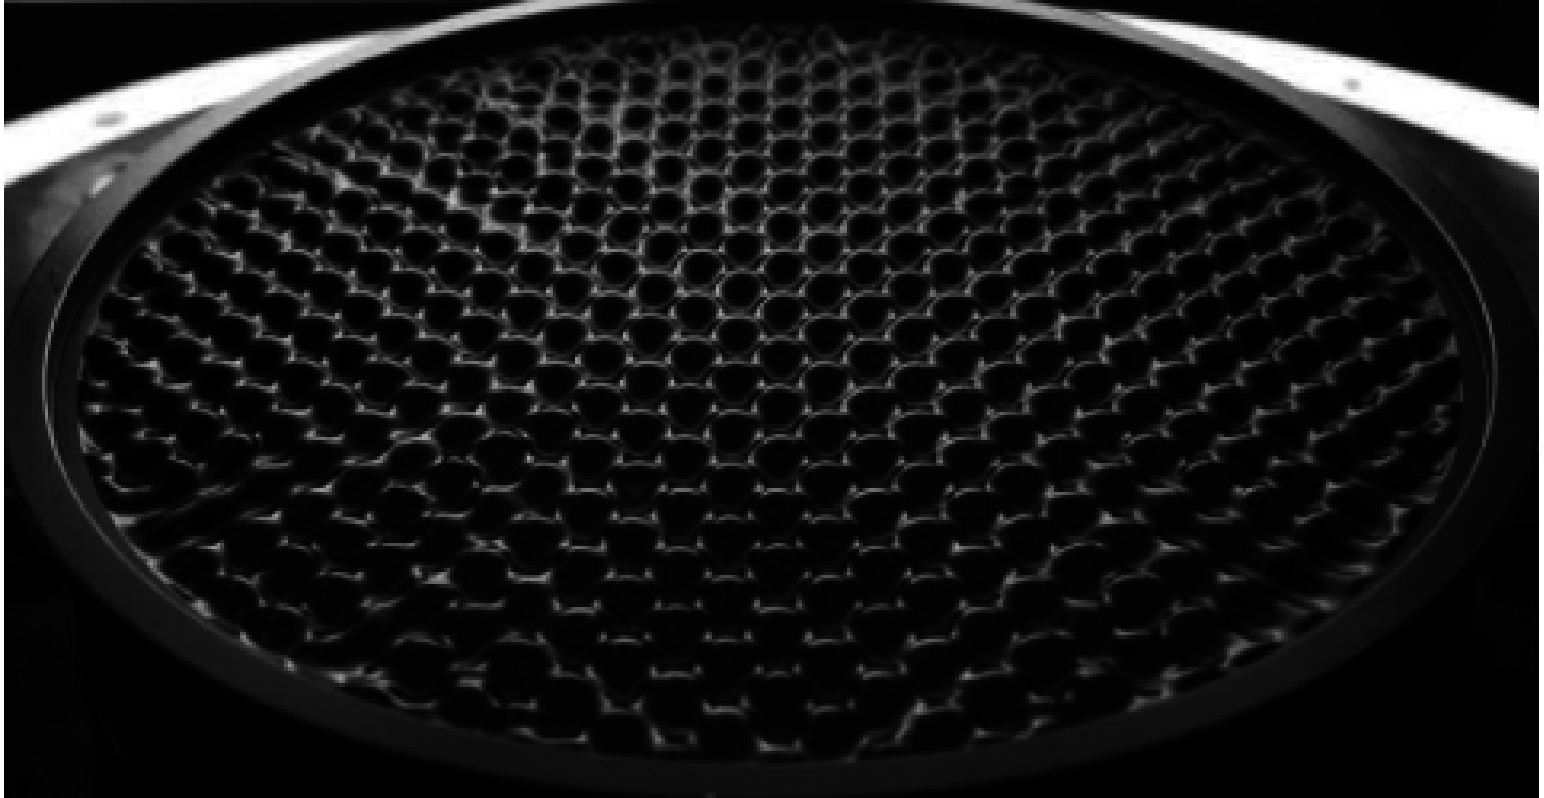
\includegraphics[width=1\textwidth]{figs/shats_snapshot_faraday_c.png}
	  \end{figure}
	\end{minipage} \hfill
	\begin{minipage}{0.3\textwidth}
	  \begin{figure}
	    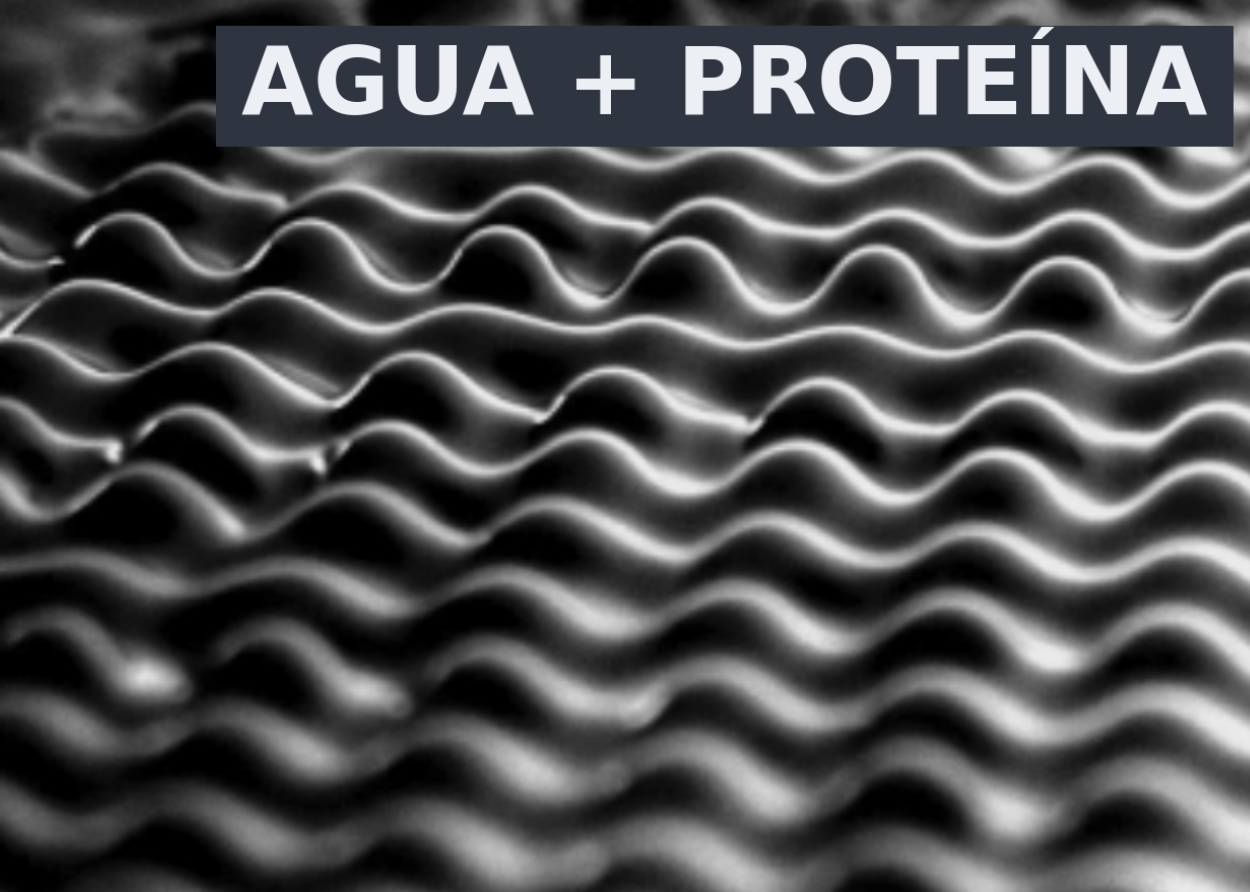
\includegraphics[width=0.9\textwidth]{figs/shats_snapshot_water+prote.png}\\
	    \vspace{0.5cm}
	     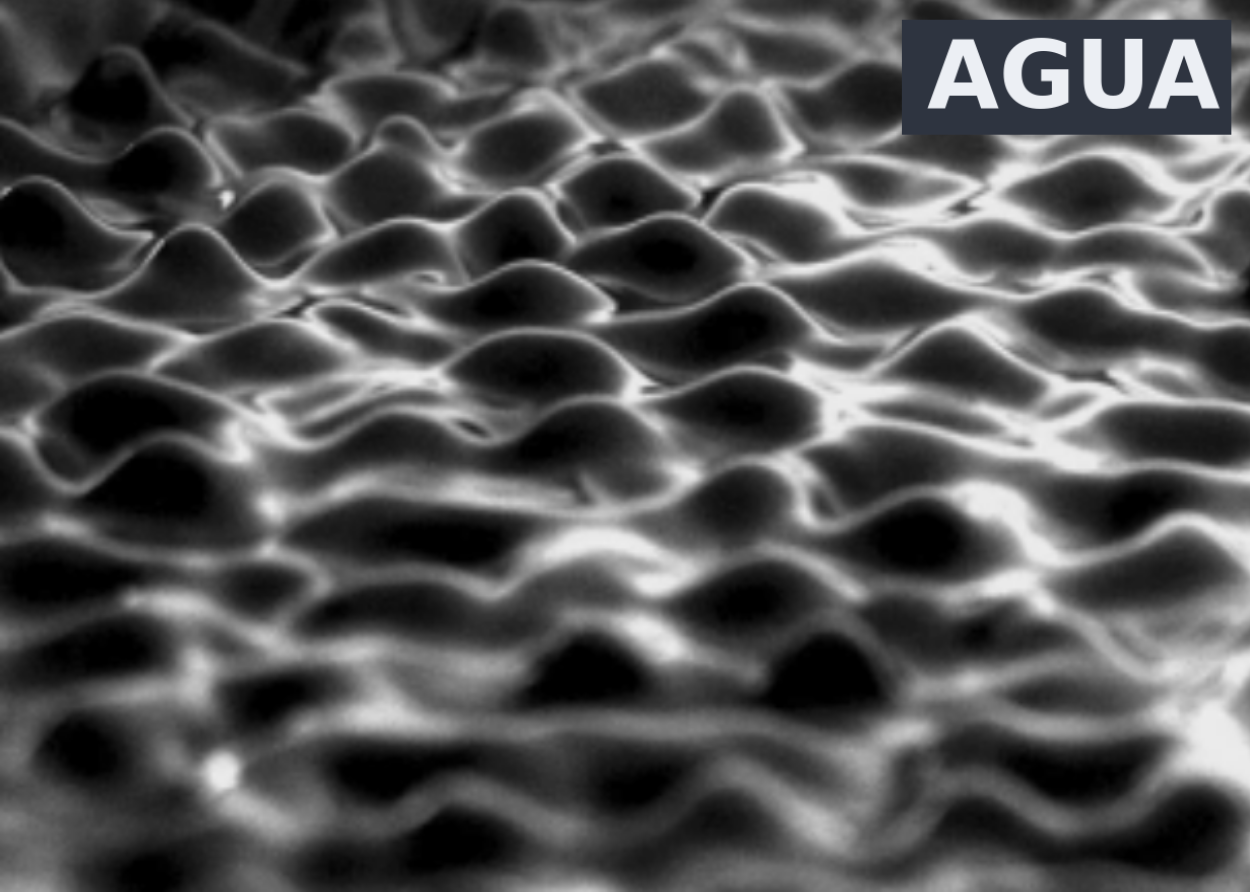
\includegraphics[width=0.9\textwidth]{figs/shats_snapshot_water.png}
	  \end{figure}
	\end{minipage}

	\hfill

	\vskip1em

	\tiny M. Shats, H. Xia, and H. Punzmann. Parametrically Excited Water Surface Ripples as Ensembles of Oscillons. Physical Review Letters, 108(3):034502, January 2012.
\end{frame}

\begin{frame}{Oscilones en 1D}
	\begin{figure}
		\centering
		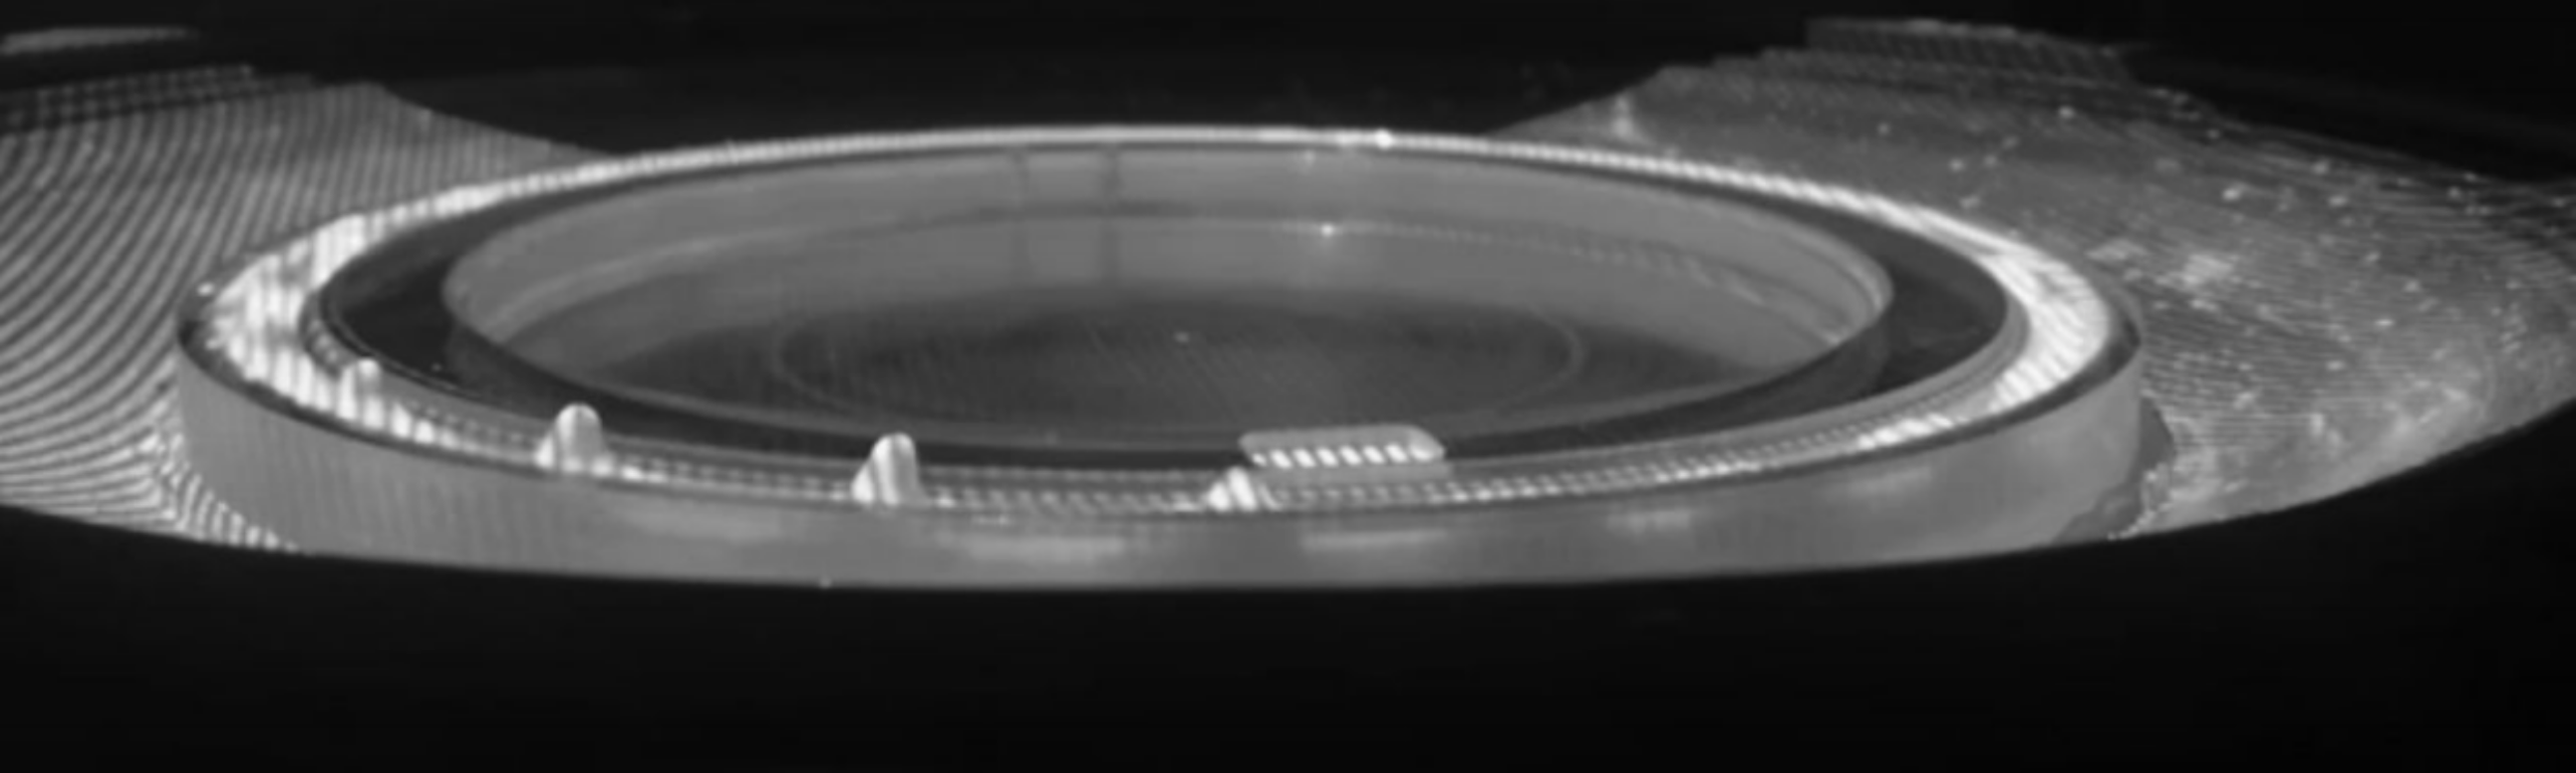
\includegraphics[height=0.28\textheight]{figs/video_1.png}
		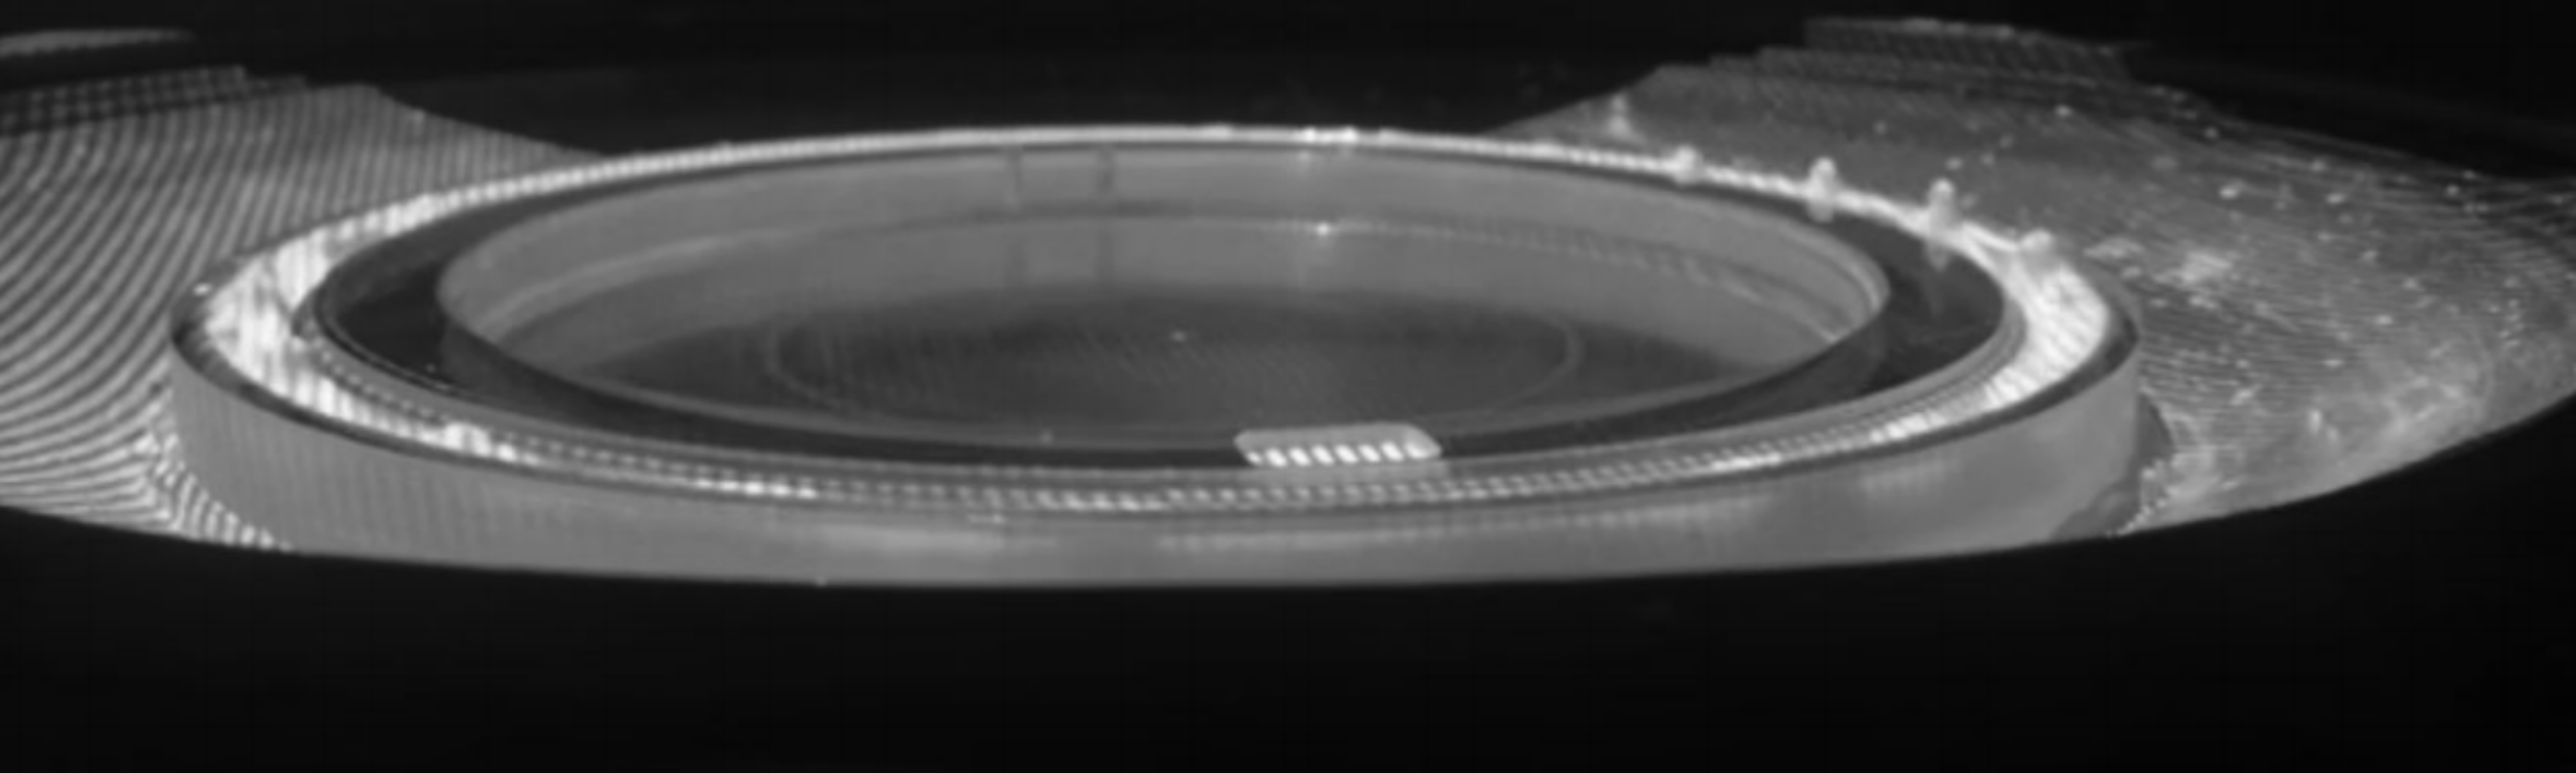
\includegraphics[height=0.28\textheight]{figs/video_2.png}
		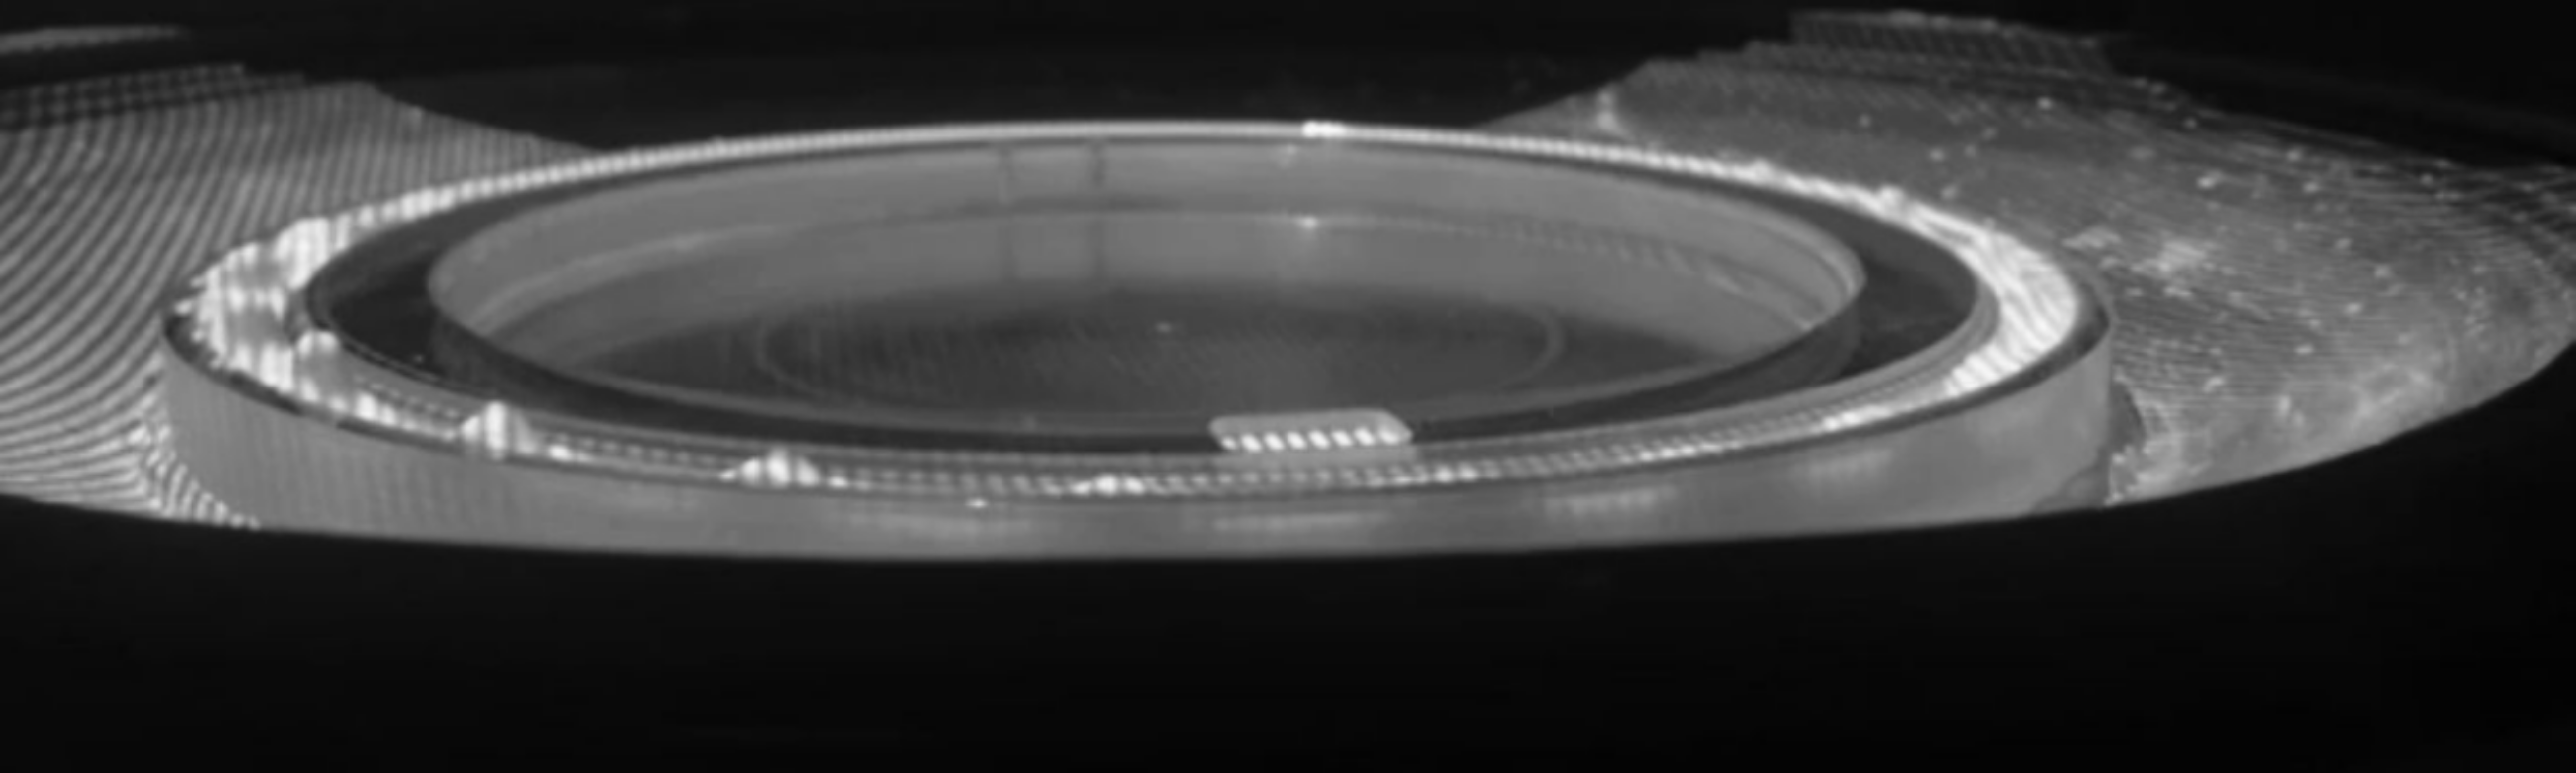
\includegraphics[height=0.28\textheight]{figs/video_3.png}
	\end{figure}
\end{frame}

\section{Montaje experimental}

\begin{frame}{Montaje experimental}
	\begin{figure}[ht]
		\centering
		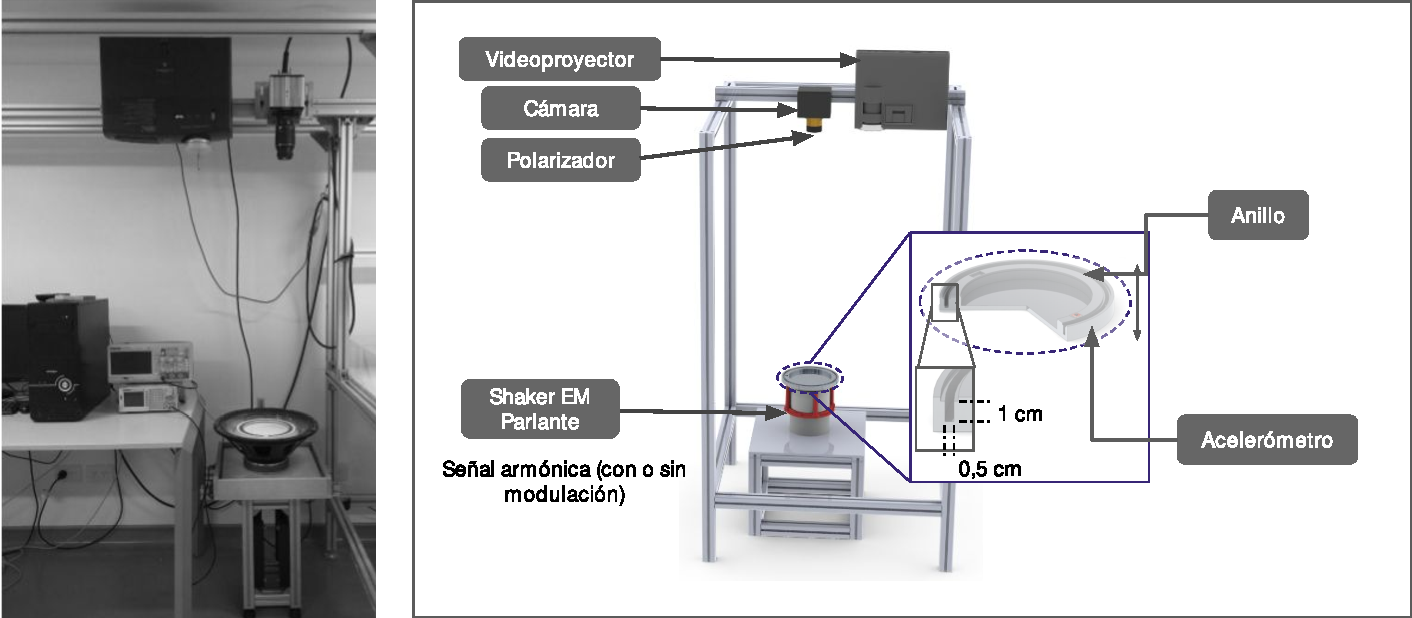
\includegraphics[width=1\textwidth]{figs/esquema_experimental.pdf}
	\end{figure}
\end{frame}

\section{Extracción de la superficie libre}

\begin{frame}{FTP}
	\begin{minipage}{0.7\textwidth}
	  \begin{figure}
		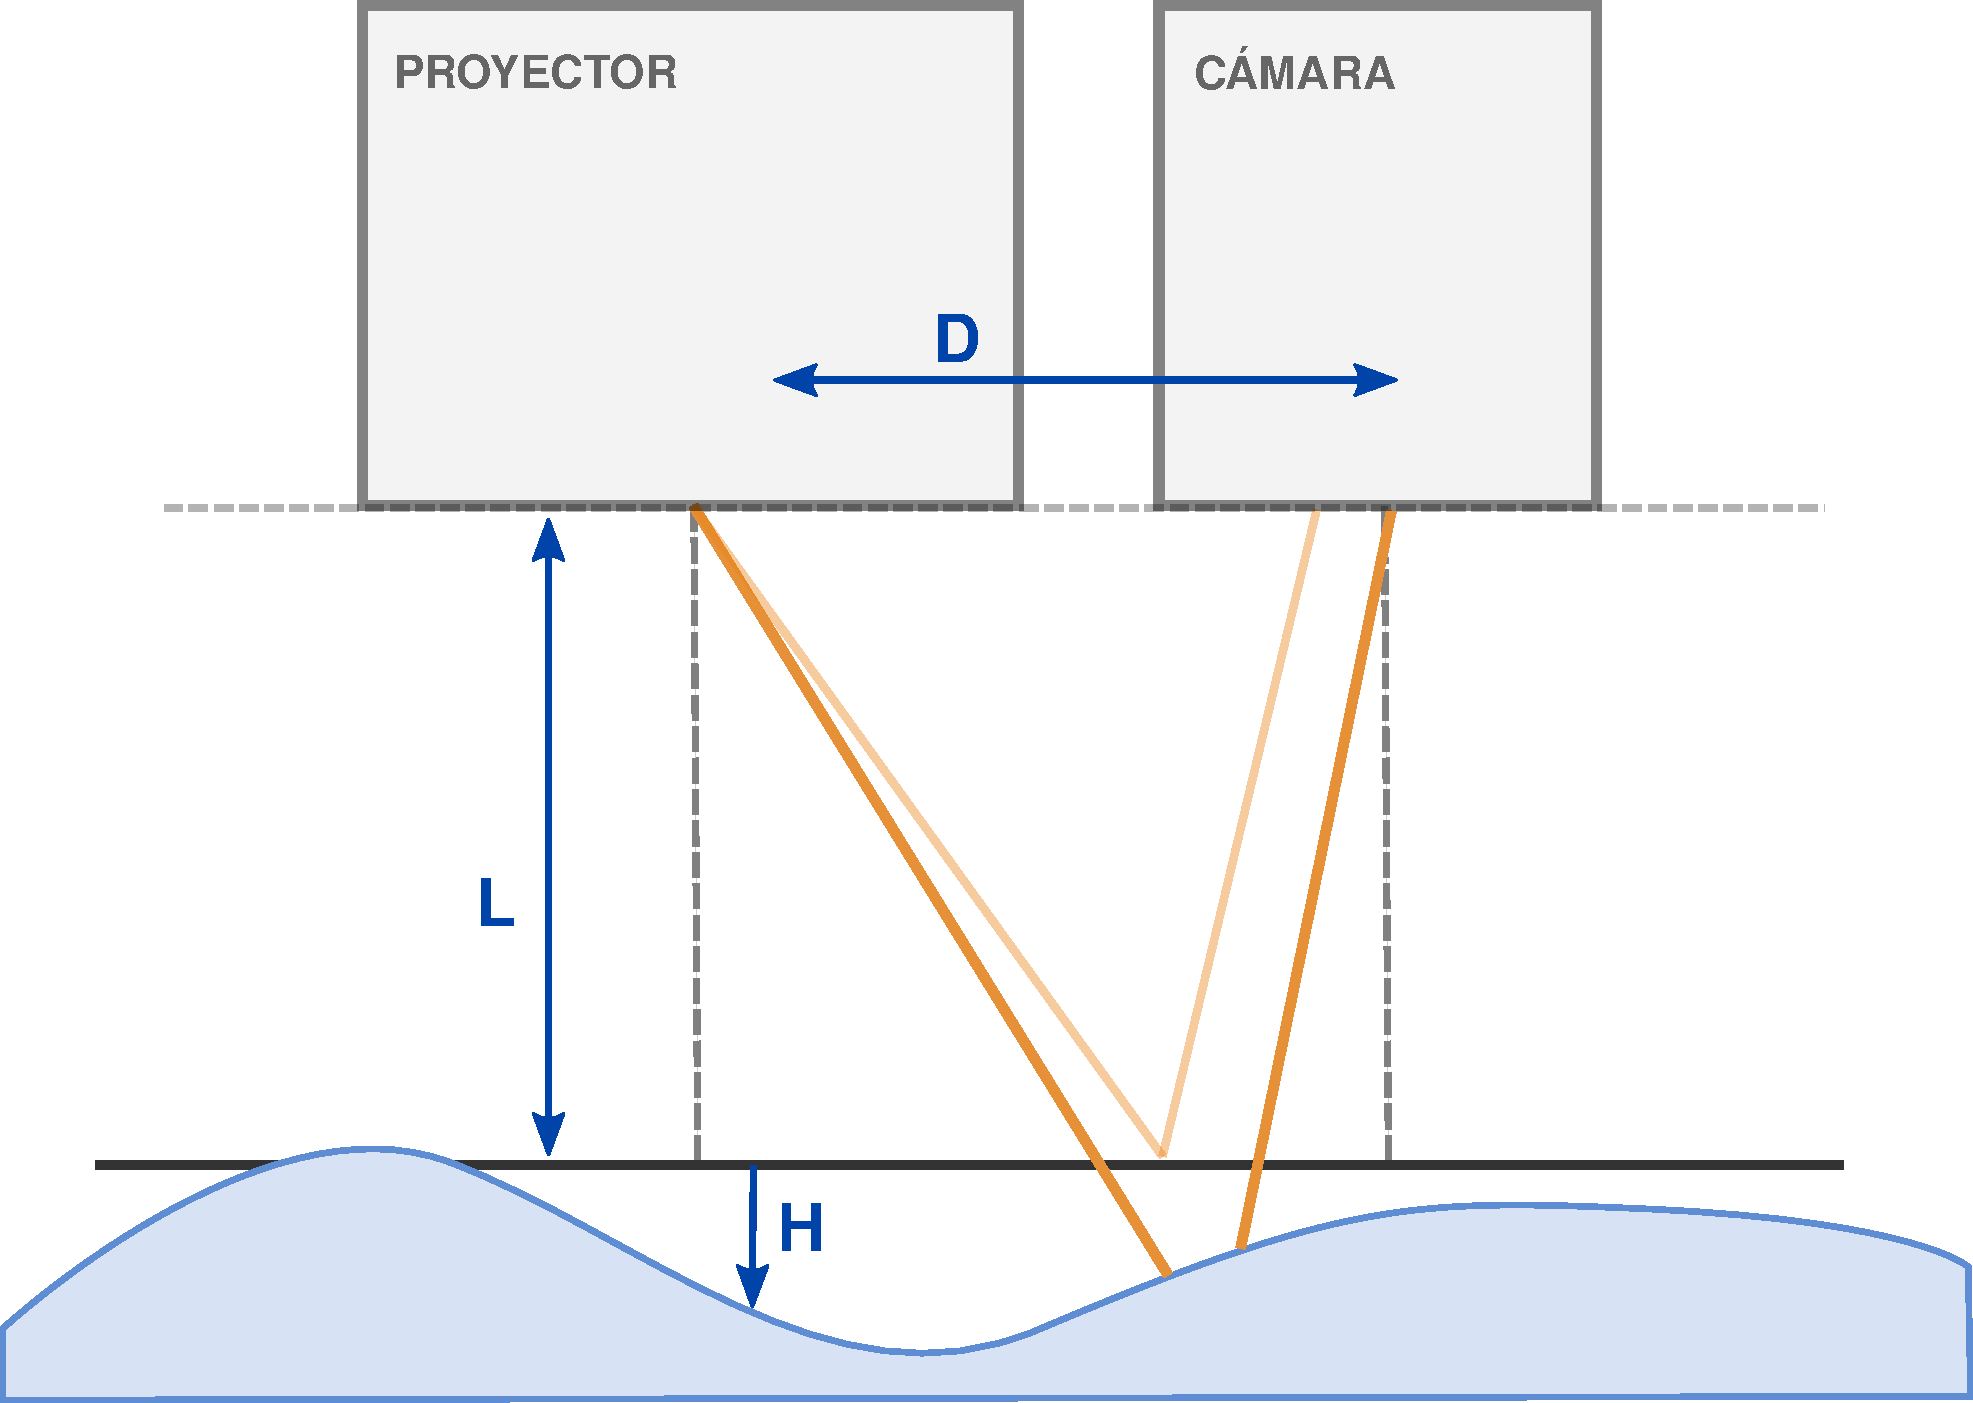
\includegraphics[width=1\textwidth]{figs/ftp_experimental.pdf}
	  \end{figure}
	\end{minipage} \hfill
	\begin{minipage}{0.29\textwidth}
	  \begin{figure}
	    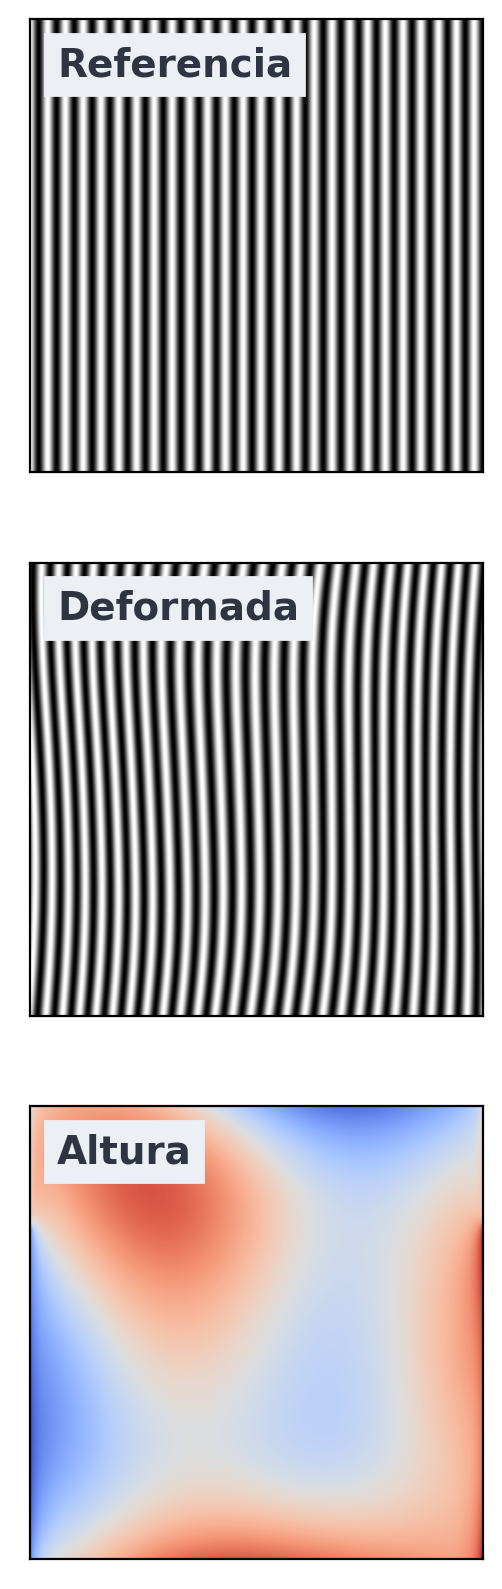
\includegraphics[width=0.56\textwidth]{figs/synthetic_ftp.png}
	  \end{figure}
	\end{minipage}
	\hfill
	\tiny P. Cobelli, A. Maurel, V. Pagneux, and P. Petitjeans. Global measurement of water waves by Fourier transform profilometry.  Experiments in Fluids, 46(6):1037–1047, 2009.
\end{frame}

\begin{frame}{Extracción de la superficie libre} % TODO
	\begin{minipage}{0.49\textwidth}
	  \begin{figure}
	    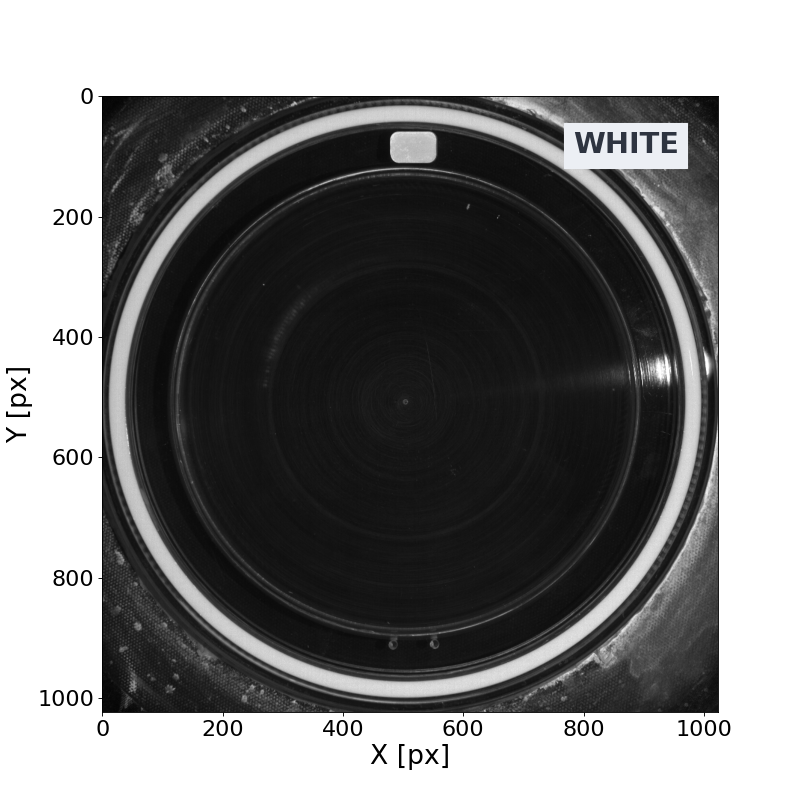
\includegraphics[width=\linewidth]{figs/ftp_white.png}
	  \end{figure}
	\end{minipage} \hfill
	\begin{minipage}{0.49\textwidth}
	  \begin{figure}
	    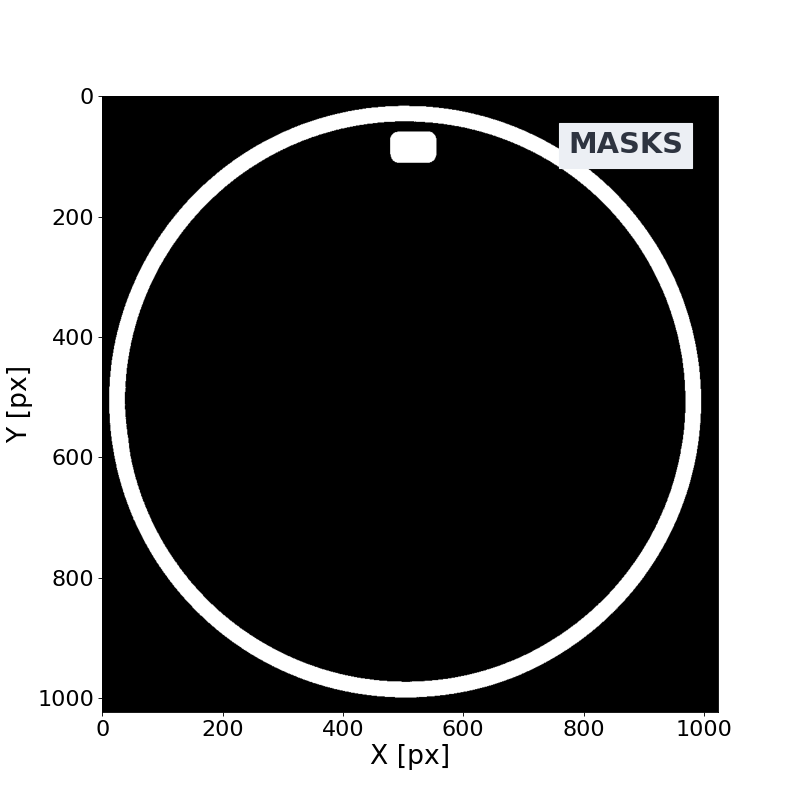
\includegraphics[width=\linewidth]{figs/ftp_masks.png}
	  \end{figure}
	\end{minipage}
	% TODO[meli]: Volver a exportar
\end{frame}

\begin{frame}{Extracción de la superficie libre} % TODO
	\begin{minipage}{0.49\textwidth}
	  \begin{figure}
	    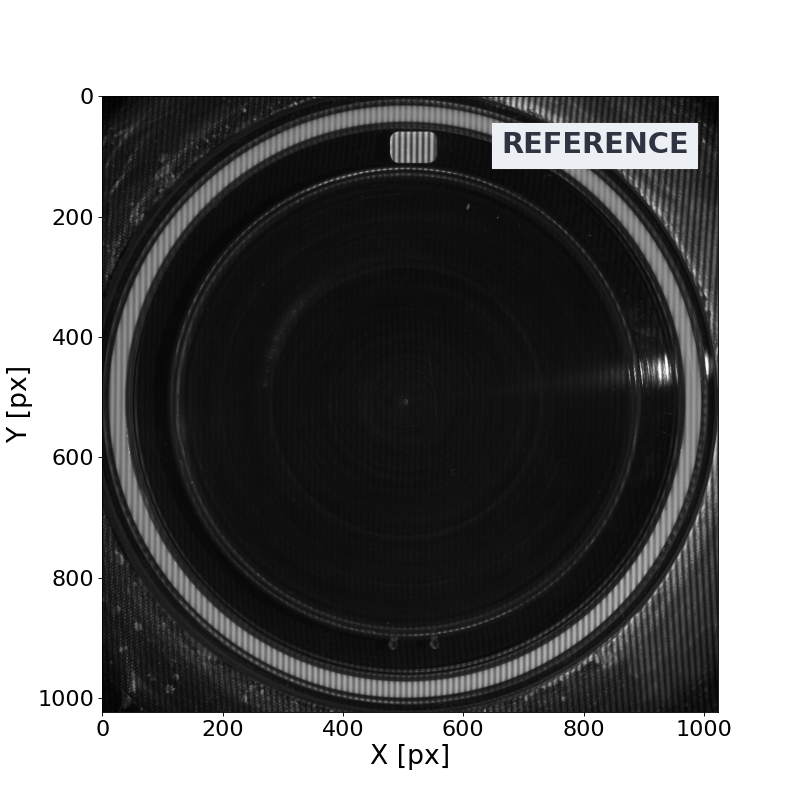
\includegraphics[width=\linewidth]{figs/ftp_reference.png}
	  \end{figure}
	\end{minipage} \hfill
	\begin{minipage}{0.49\textwidth}
	  \begin{figure}
	    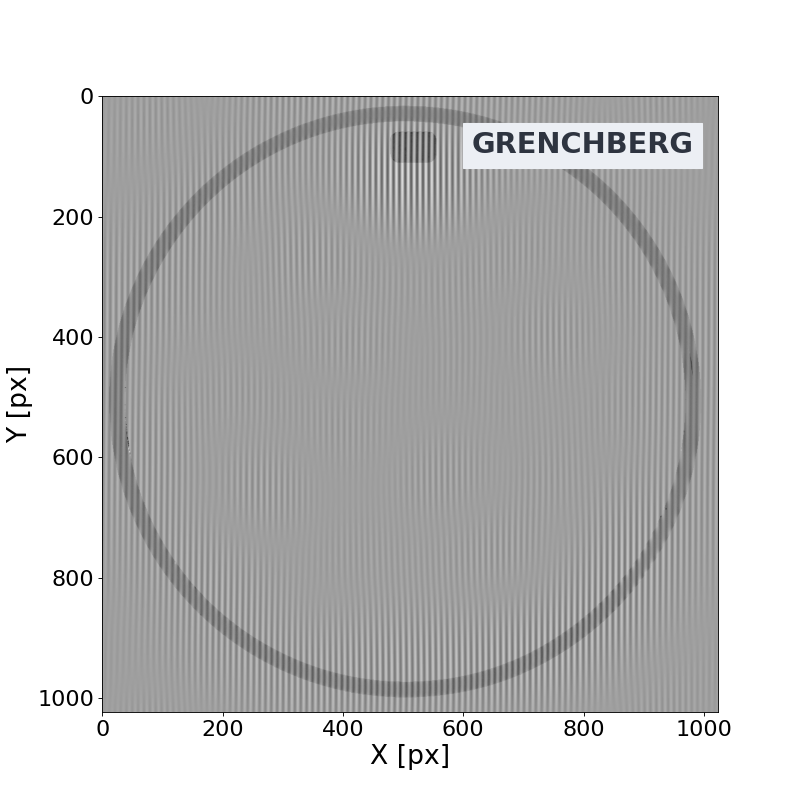
\includegraphics[width=\linewidth]{figs/ftp_gerchberg.png}
	  \end{figure}
	\end{minipage}
	% TODO[meli]: Volver a exportar
\end{frame}

\begin{frame}{Extracción de la superficie libre} % TODO
	\begin{minipage}{0.49\textwidth}
	  \begin{figure}
	    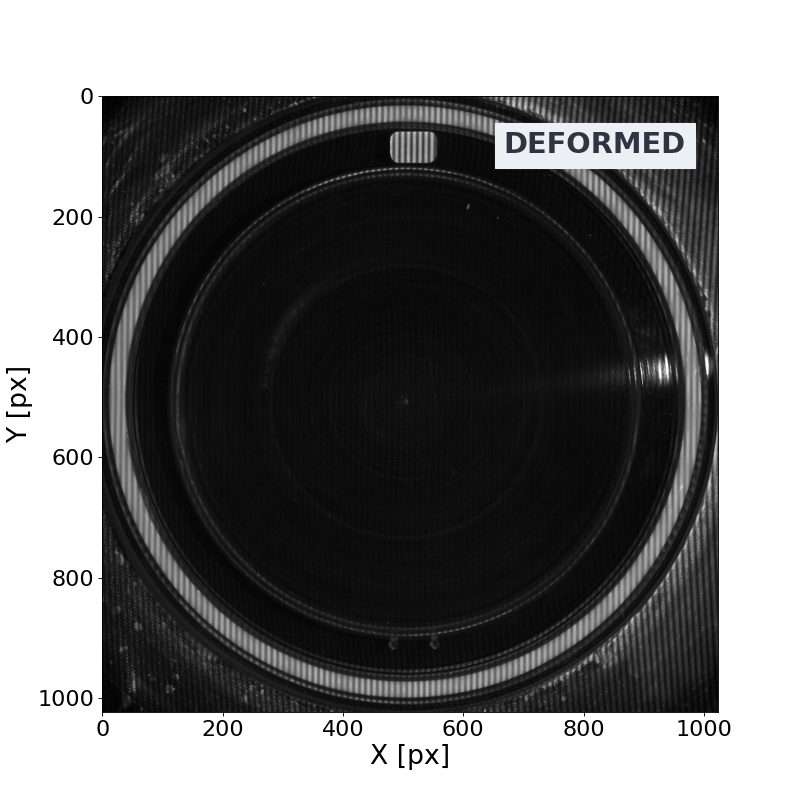
\includegraphics[width=\linewidth]{figs/ftp_deformed.png}
	  \end{figure}
	\end{minipage} \hfill
	\begin{minipage}{0.49\textwidth}
	  \begin{figure}
	    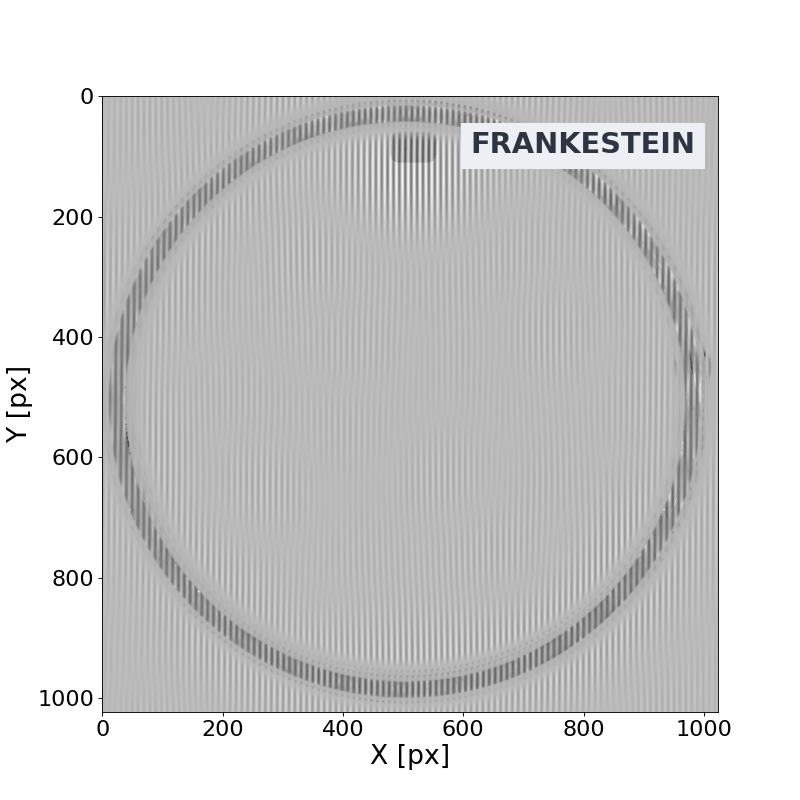
\includegraphics[width=\linewidth]{figs/ftp_hybrid.png}
	  \end{figure}
	\end{minipage}
	% TODO[meli]: Volver a exportar
\end{frame}

\begin{frame}{Extracción de la superficie libre} % TODO
	\begin{minipage}{0.49\textwidth}
	  \begin{figure}
	    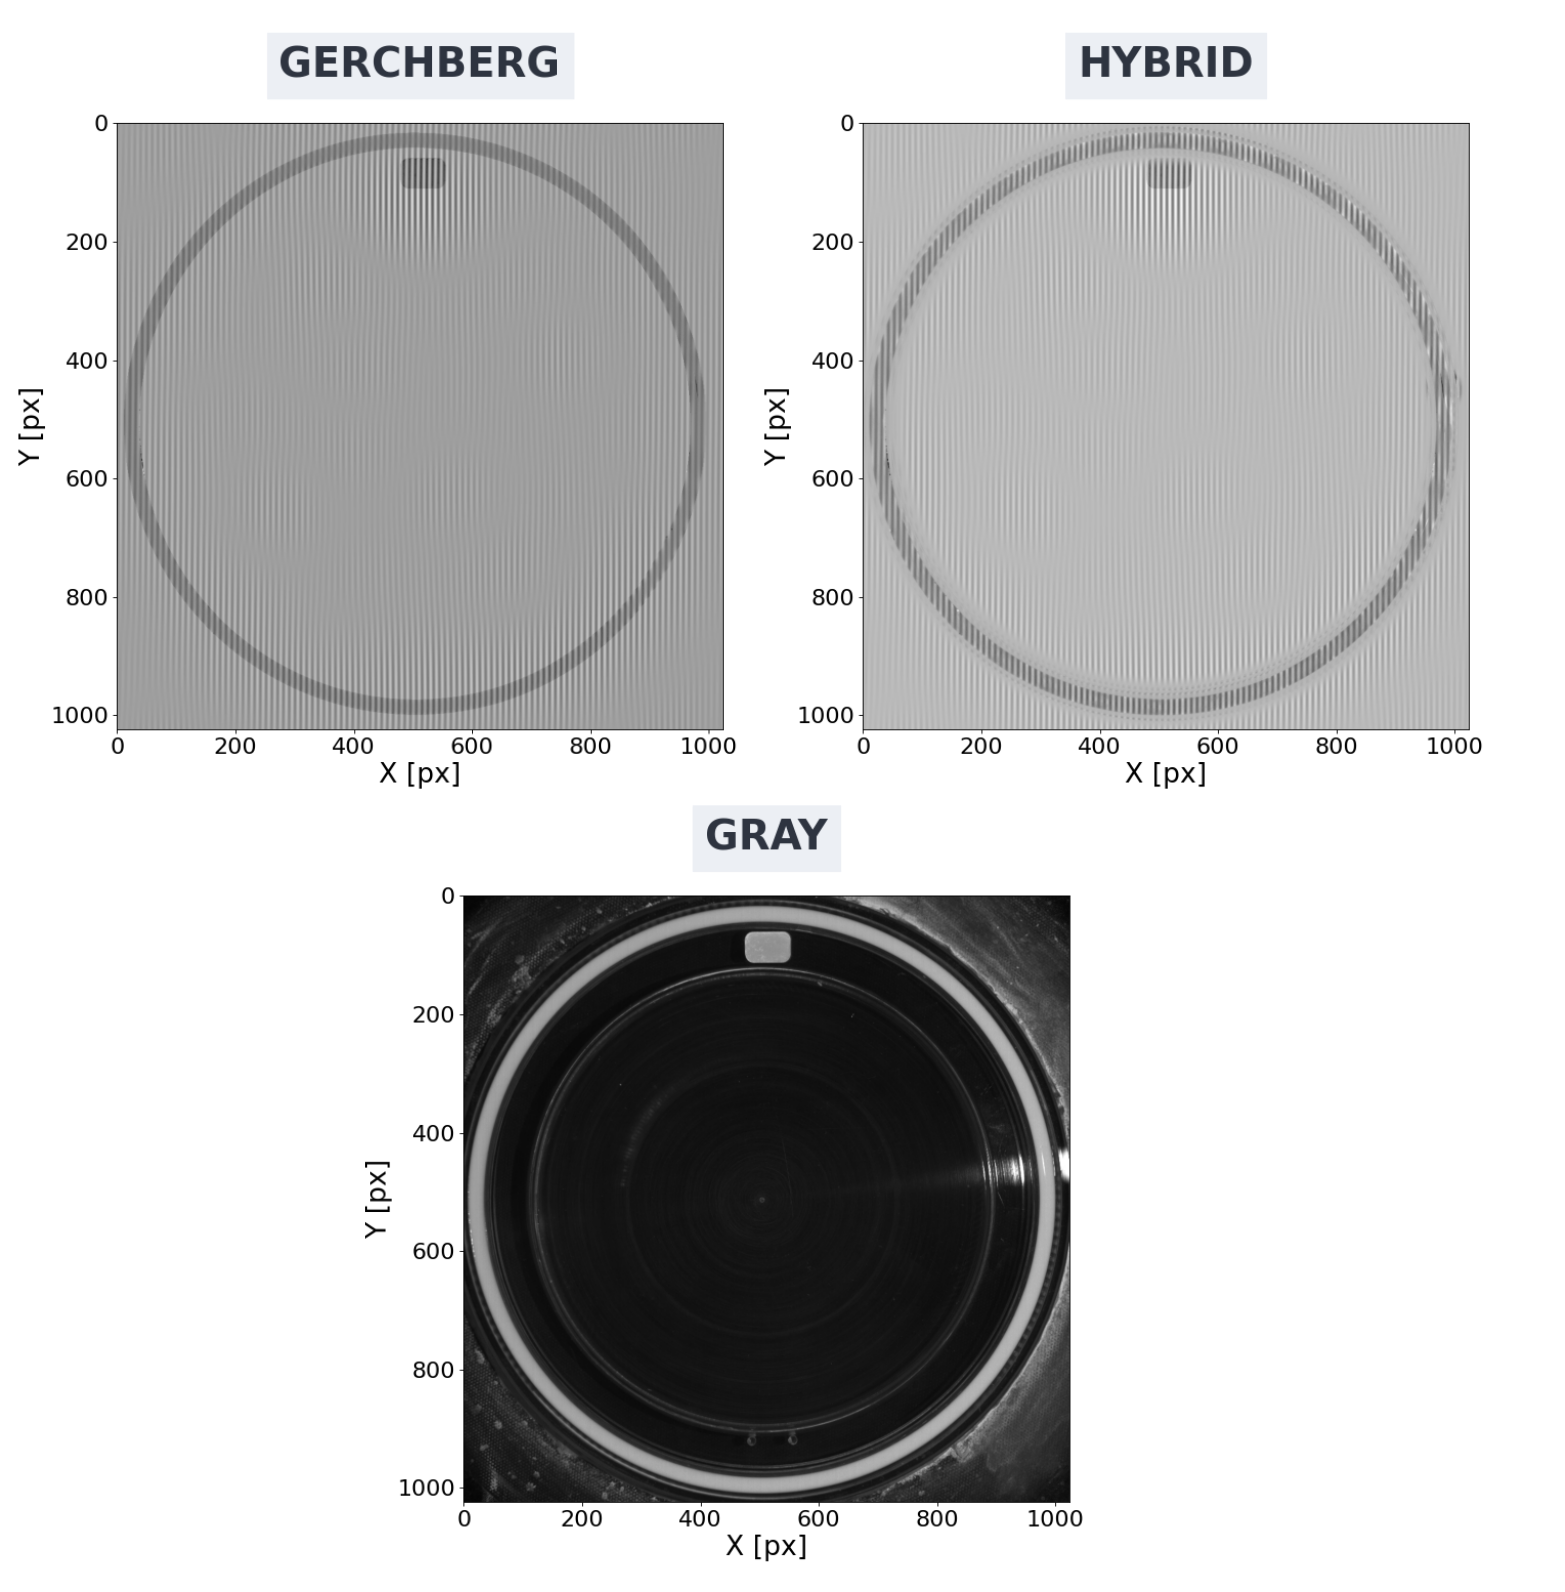
\includegraphics[width=0.85\linewidth]{figs/ftp_collage.png}
	  \end{figure}
	\end{minipage} \hfill
	\begin{minipage}{0.49\textwidth}
	  \begin{figure}
	    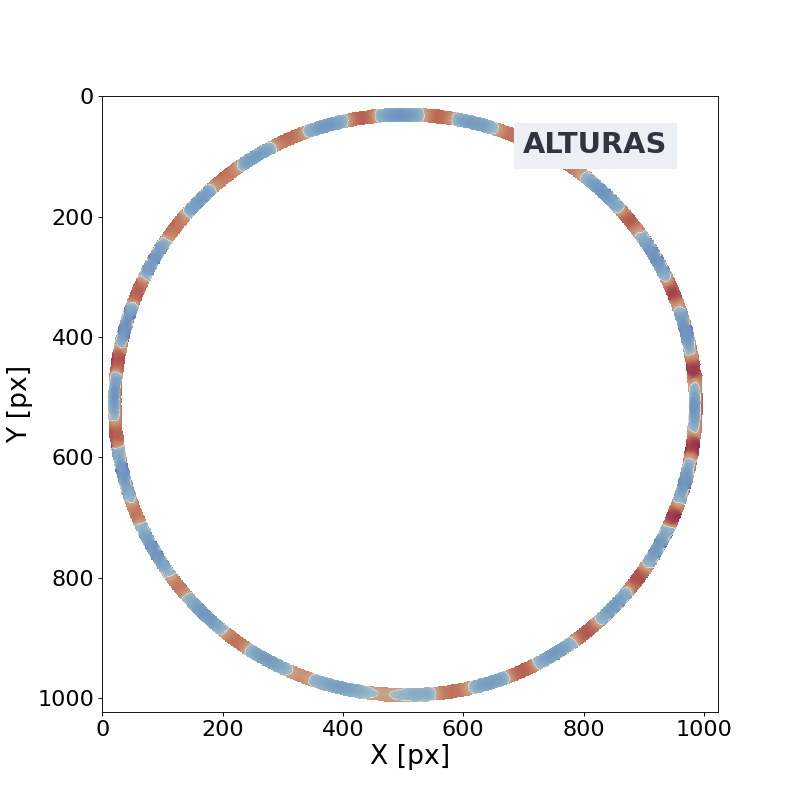
\includegraphics[width=\linewidth]{figs/ftp_alturas.png}
	  \end{figure}
	\end{minipage}
	% TODO[meli]: Volver a exportar
\end{frame}


\begin{frame}{Extracción de la superficie libre} % TODO
	\begin{minipage}{0.49\textwidth}
	  \begin{figure}
	    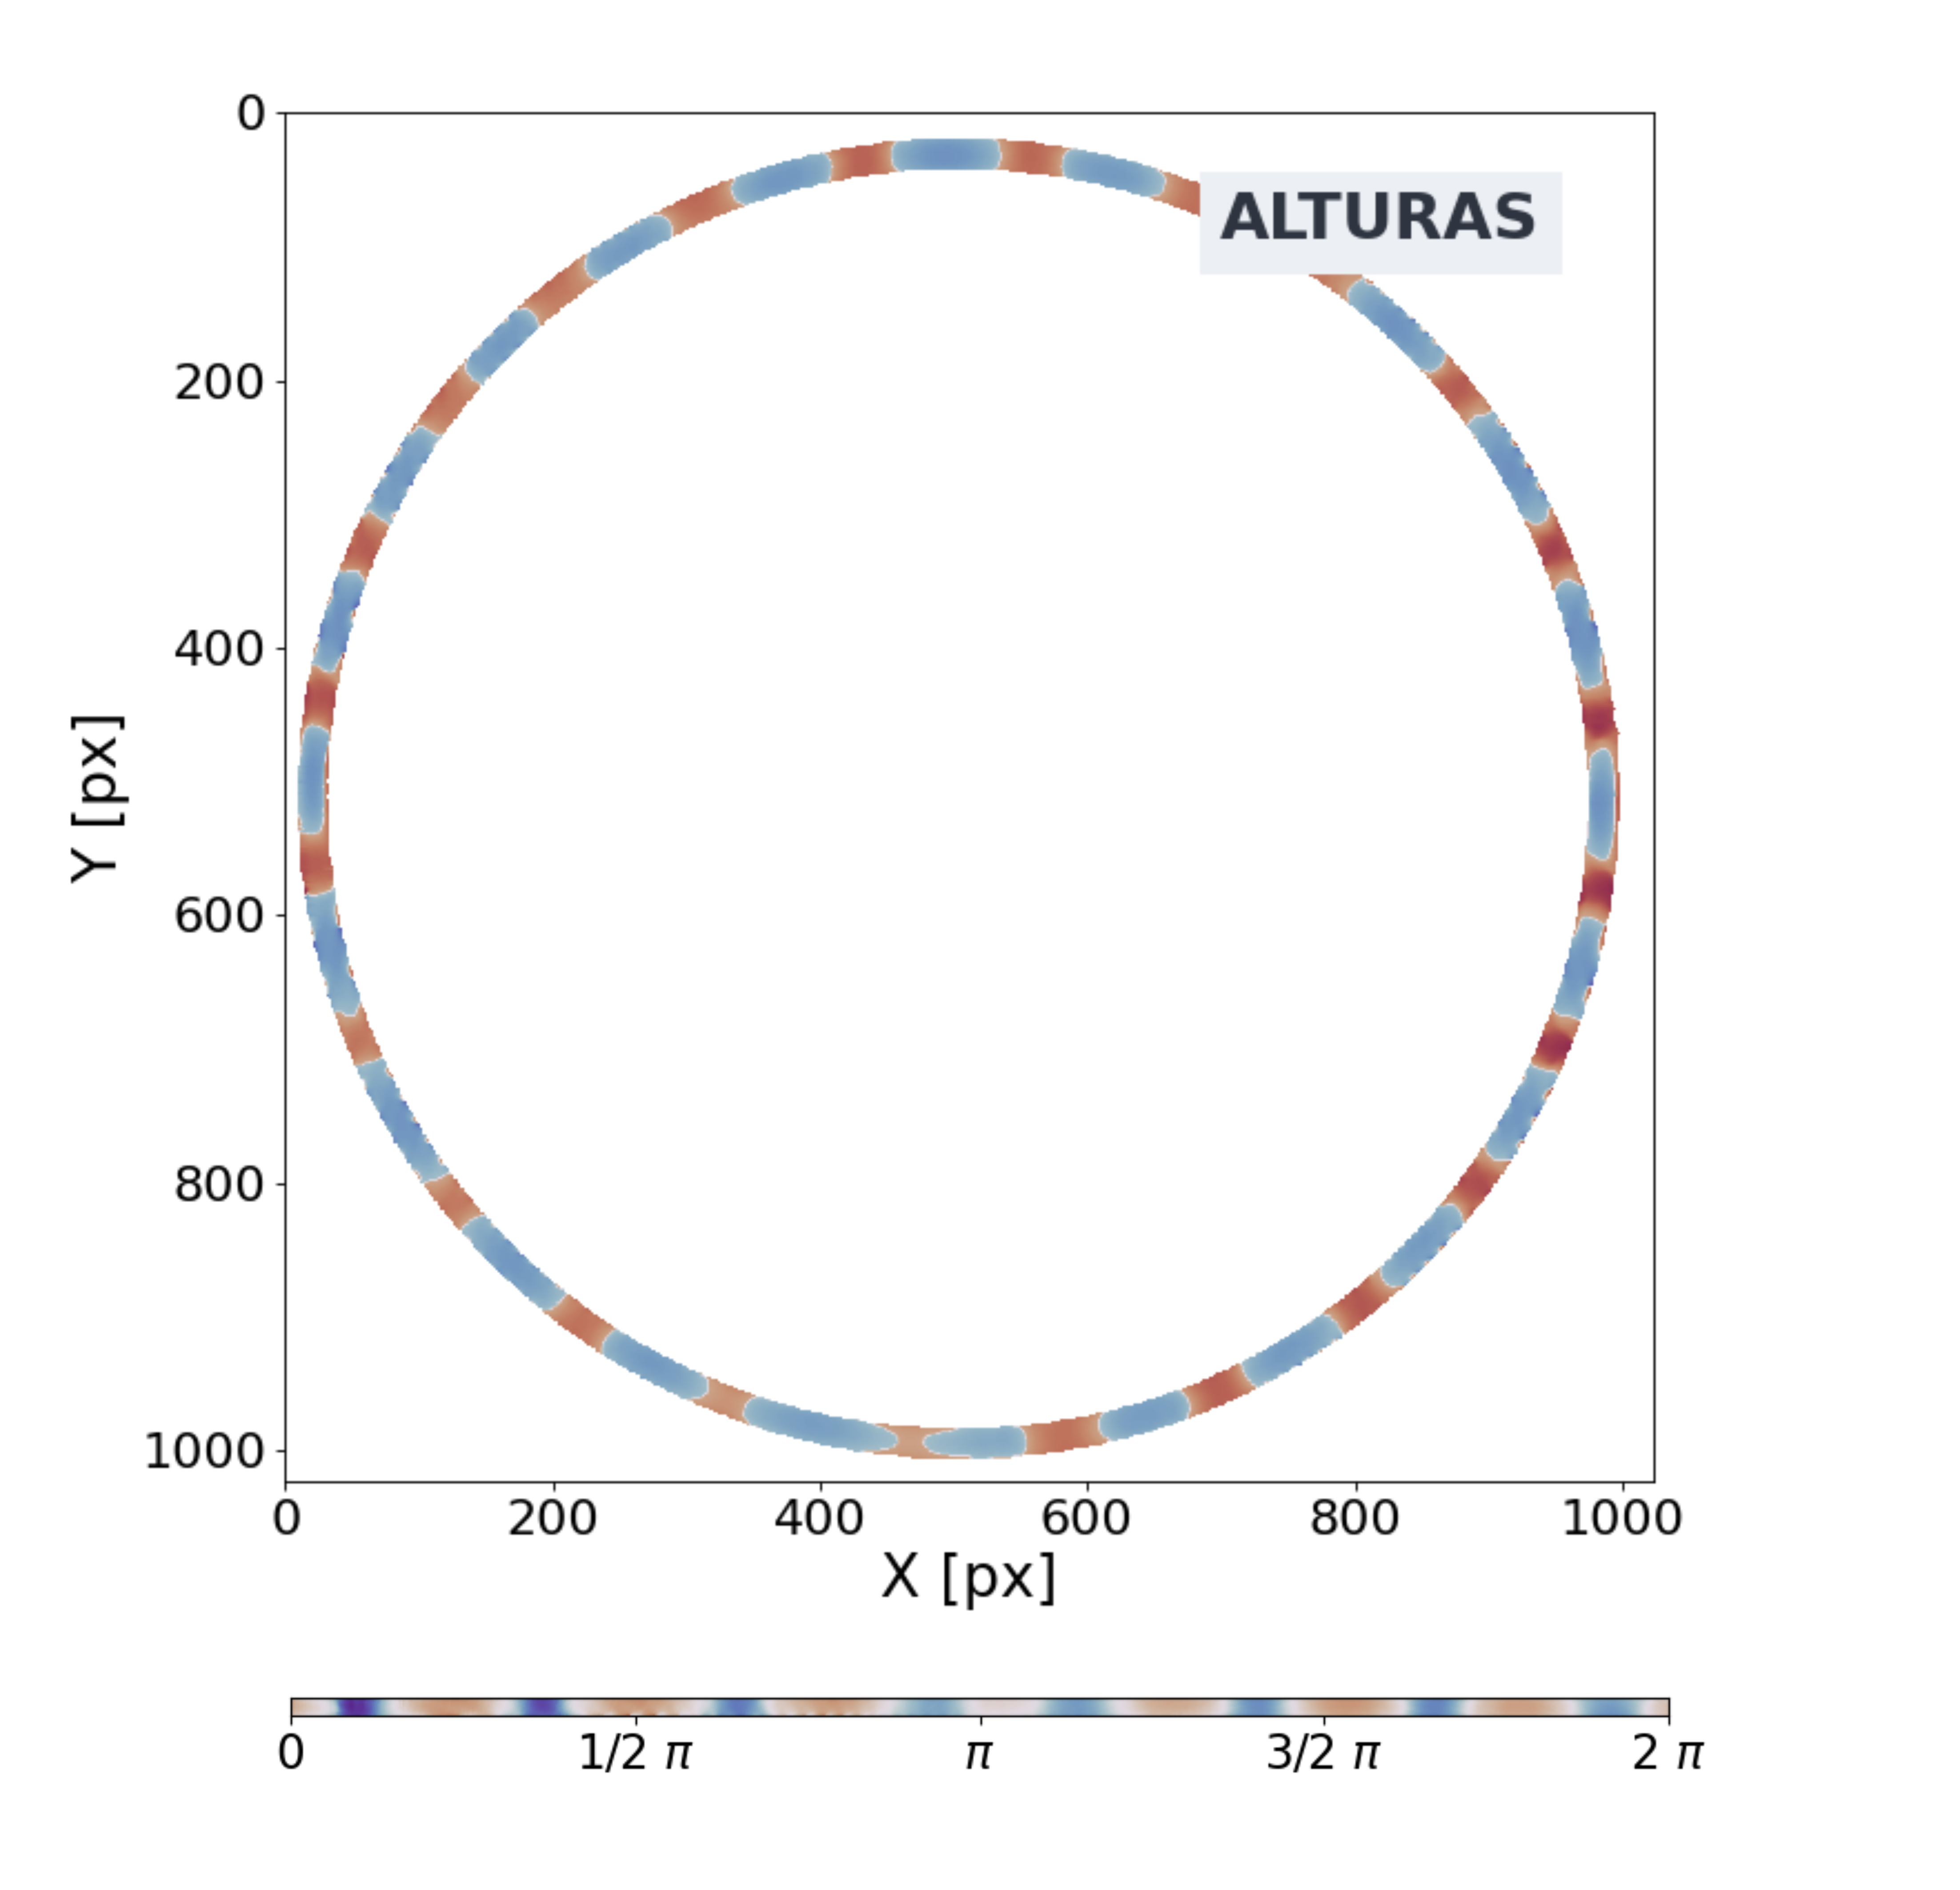
\includegraphics[width=\linewidth]{figs/annulus_to_strip.png}
	  \end{figure}
	\end{minipage} \hfill
	\begin{minipage}{0.49\textwidth}
	  \begin{figure}
	    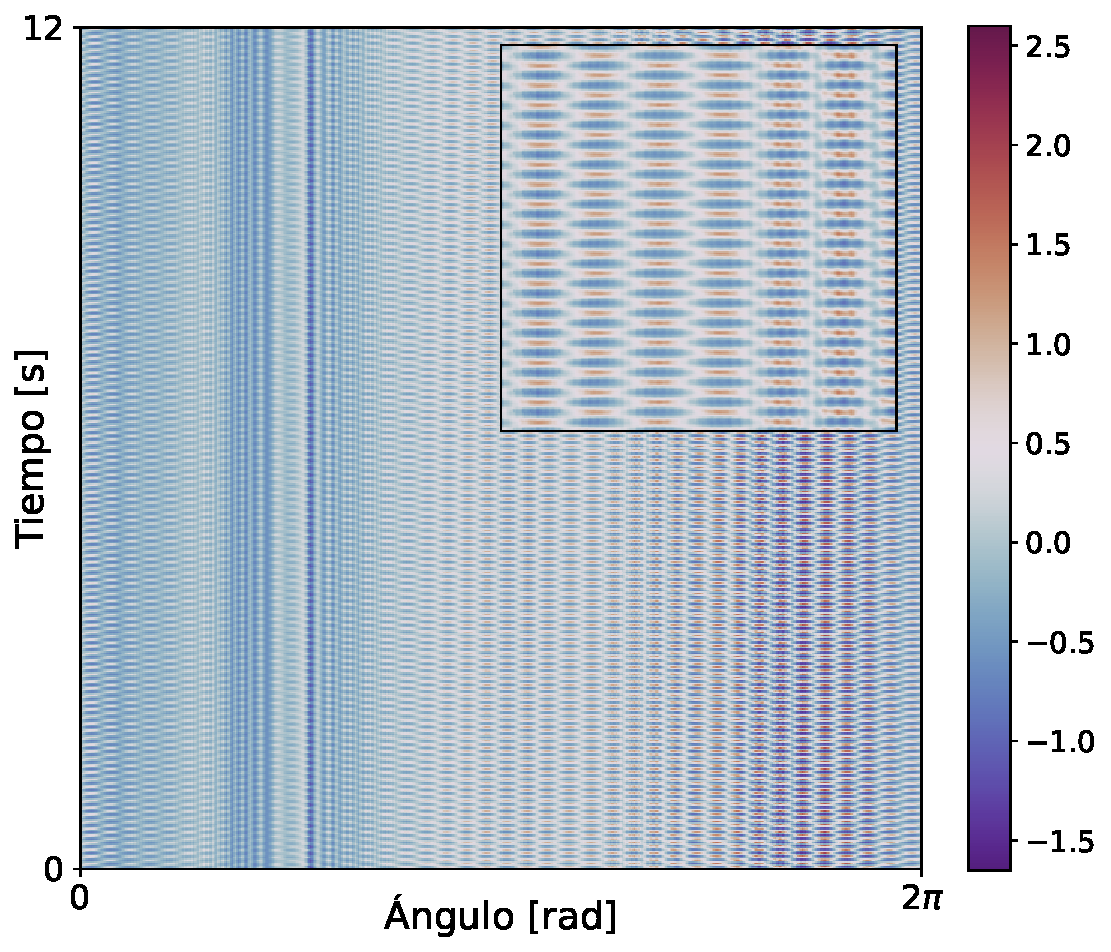
\includegraphics[width=\linewidth]{figs/st_med_example.pdf}
	  \end{figure}
	\end{minipage}
	% TODO[meli]: Volver a exportar
\end{frame}

\begin{frame}{Manejo de archivos y HDF5}
	\begin{figure}
		\centering
		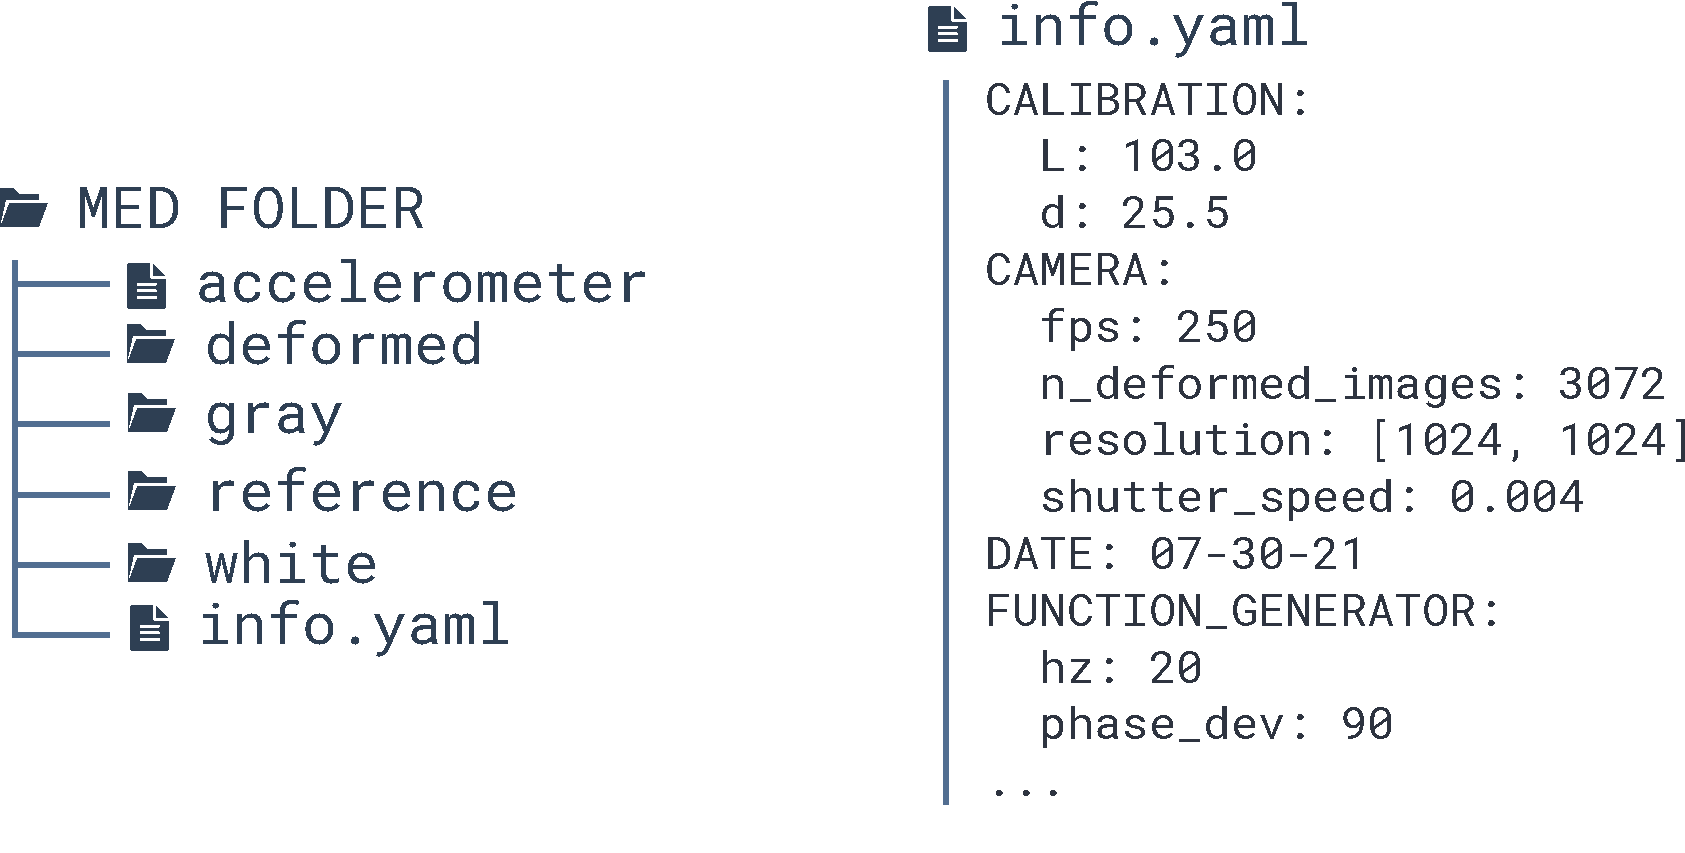
\includegraphics[width=1\textwidth]{figs/med_folder_infoyaml.pdf}
	\end{figure}
\end{frame}


\begin{frame}{Algunas métricas} % TODO
	\begin{itemize}
		\item 70 mediciones
		\item Videos de $12\text{s}$ de medición a $250\text{fps}$ 
		\item Fotogramas de $(1024\cross1024)\text{px}$
		\item Espacio en memoria para cada medición
			\begin{itemize}
				\item $4\text{GB}$ (mediciones crudas)
				\item $40\text{GB}$ (mediciones procesadas) (HDF5)
				\item $100\text{MB}$ (espacio-temporal) (HDF5)
			\end{itemize}
		\item Tiempo de ejecución: $1\text{h} \rightarrow 10\text{min}$
	\end{itemize}
\end{frame}


\section{Resultados}

\begin{frame}{Comportamientos generales estudiados}
	\begin{minipage}{0.30\textwidth}
	  \begin{figure}
		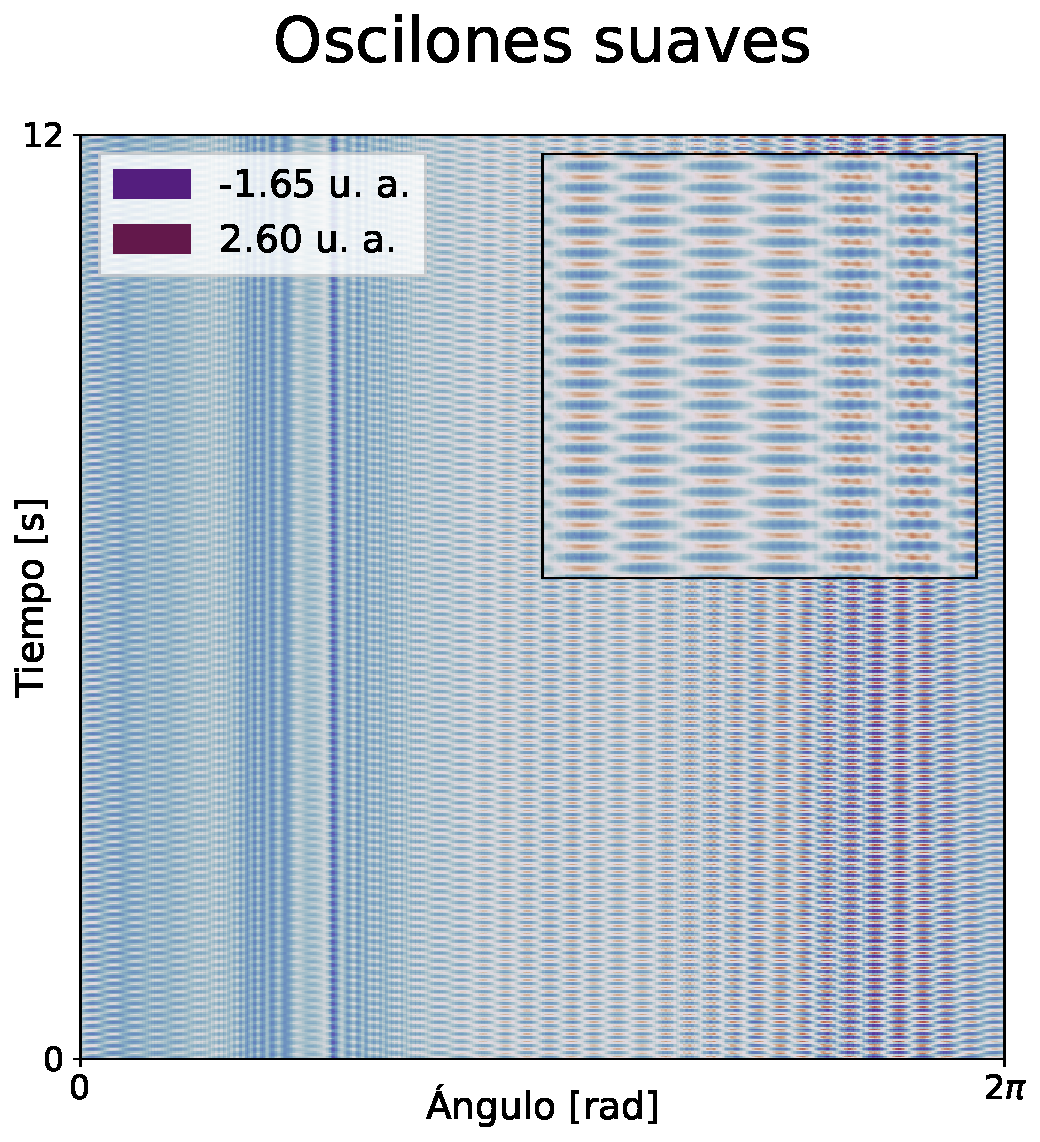
\includegraphics[width=\linewidth]{figs/st_zoologia_oscilones_suaves.pdf}
	  \end{figure}
	\end{minipage} \hfill
	\begin{minipage}{0.30\textwidth}
	  \begin{figure}
		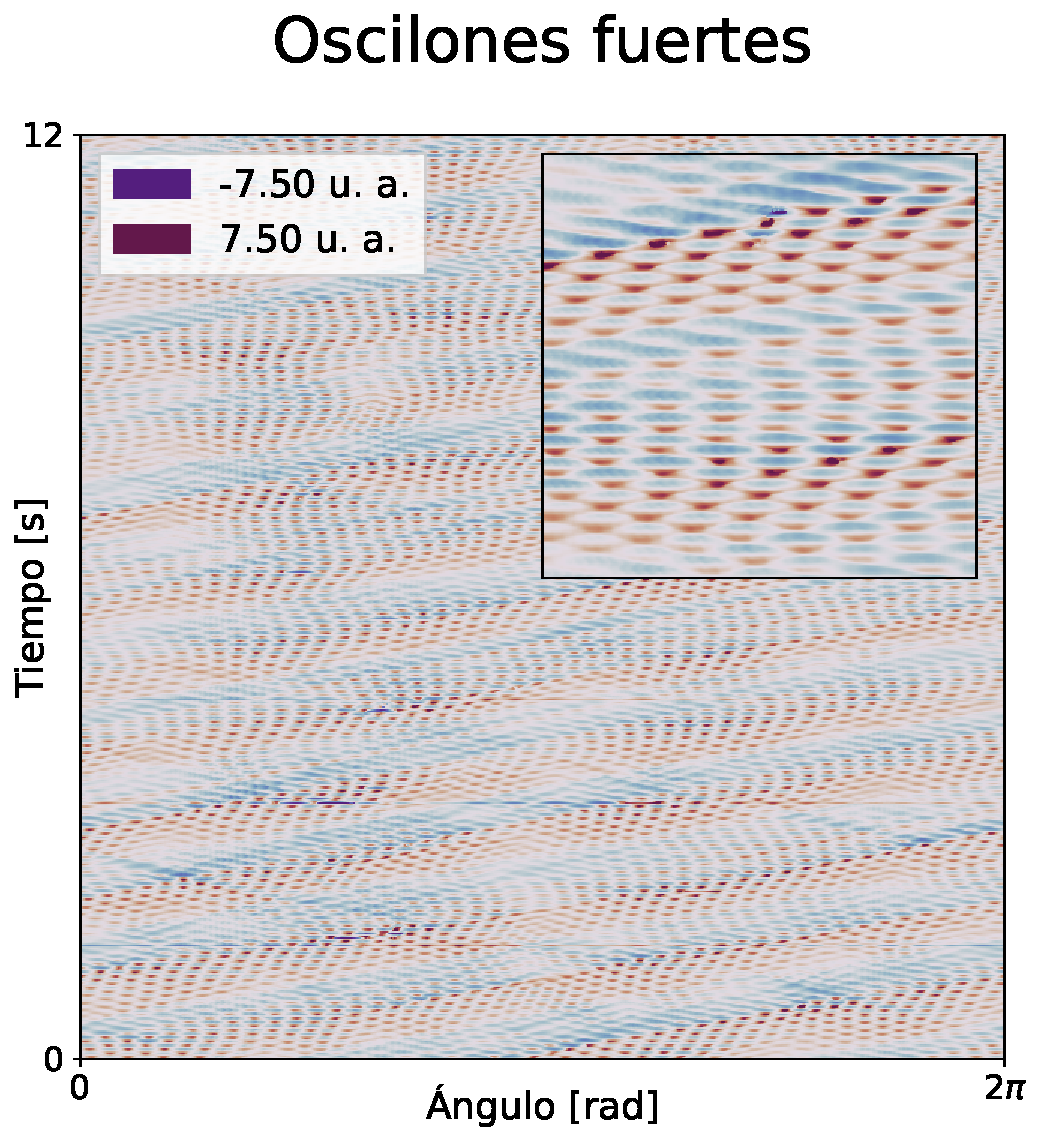
\includegraphics[width=\linewidth]{figs/st_zoologia_oscilones_fuertes.pdf}
	  \end{figure}
	\end{minipage} \hfill
	\begin{minipage}{0.30\textwidth}
	  \begin{figure}
		\includegraphics[width=\linewidth]{figs/st_zoologia_modulación_de_fase.pdf}
	  \end{figure}
	\end{minipage}
\end{frame}

\begin{frame}{Ajuste de oscilones} % TODO (2 diapos): Un solo oscilón y todos juntos
	\begin{minipage}{0.46\textwidth}
	  \begin{figure}
	    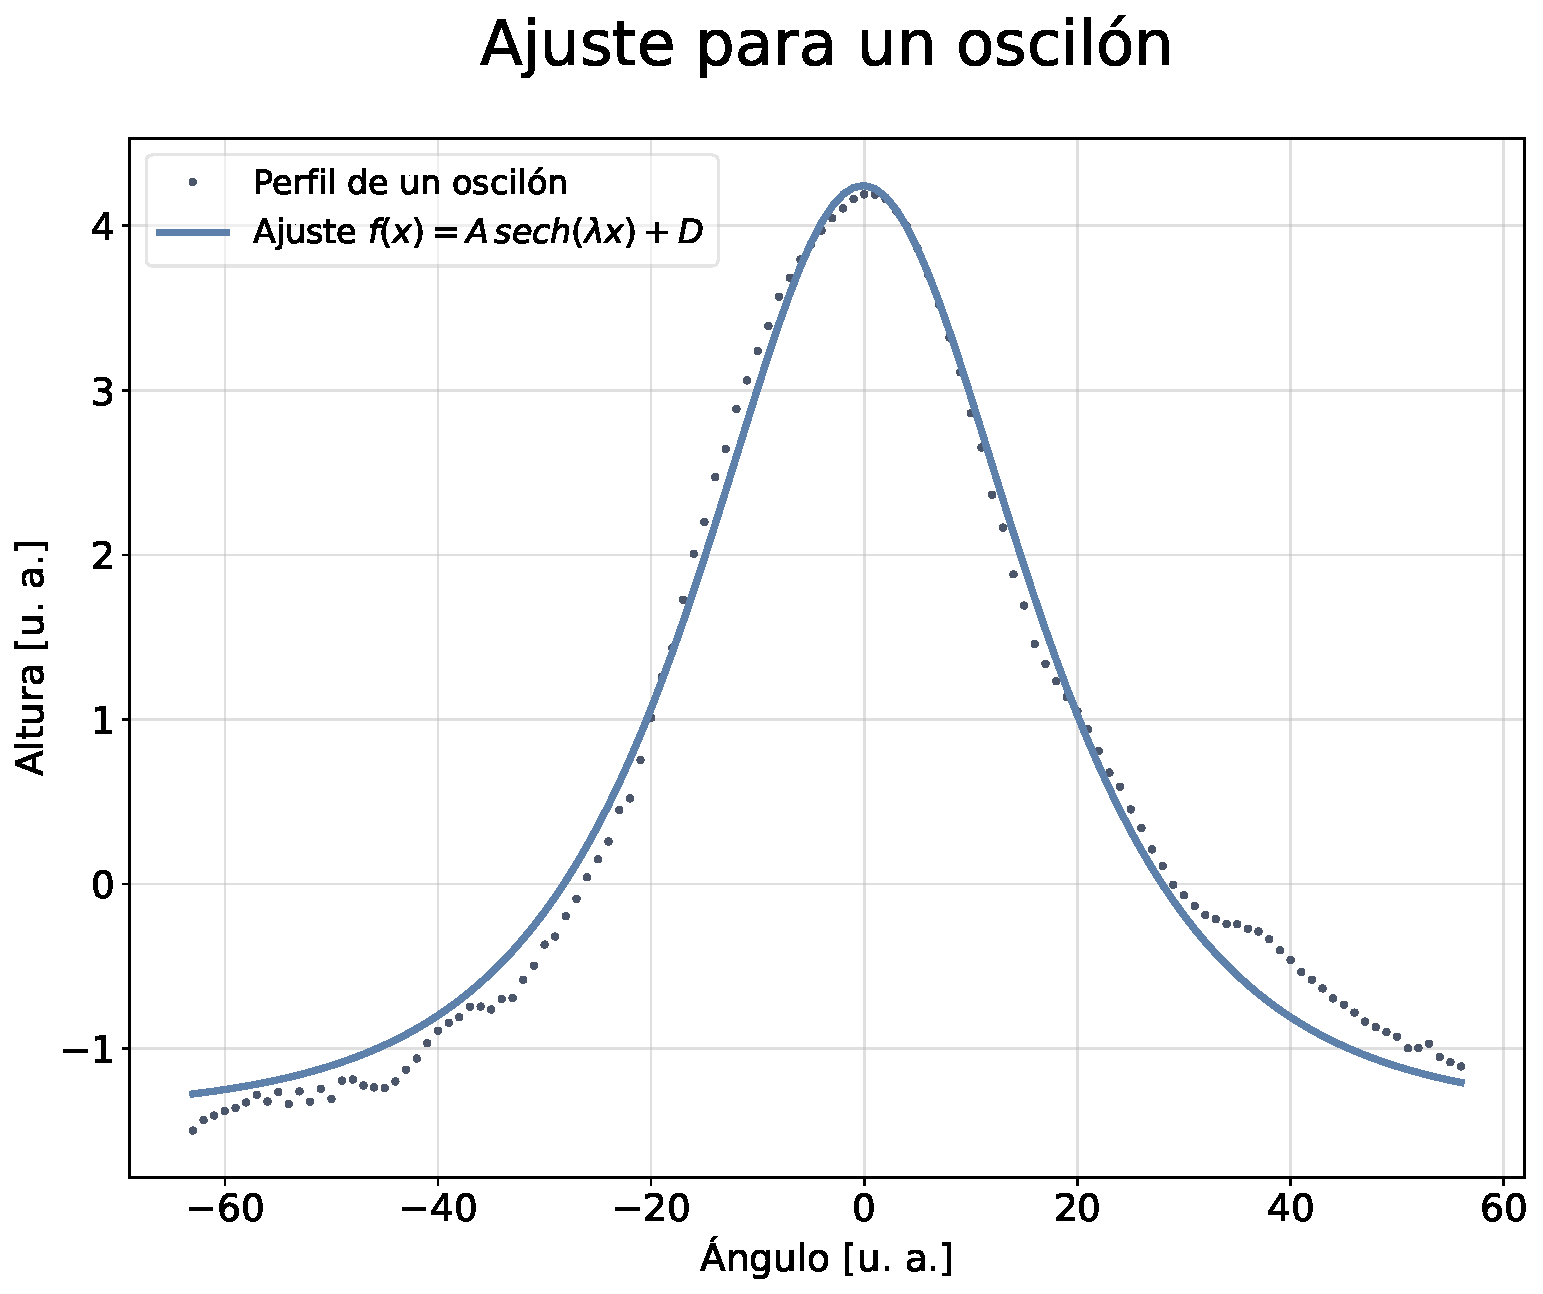
\includegraphics[width=\linewidth]{figs/fit_one_osc.pdf}
	  \end{figure}
	\end{minipage} \hfill
	\begin{minipage}{0.46\textwidth}
	  \begin{figure}
	    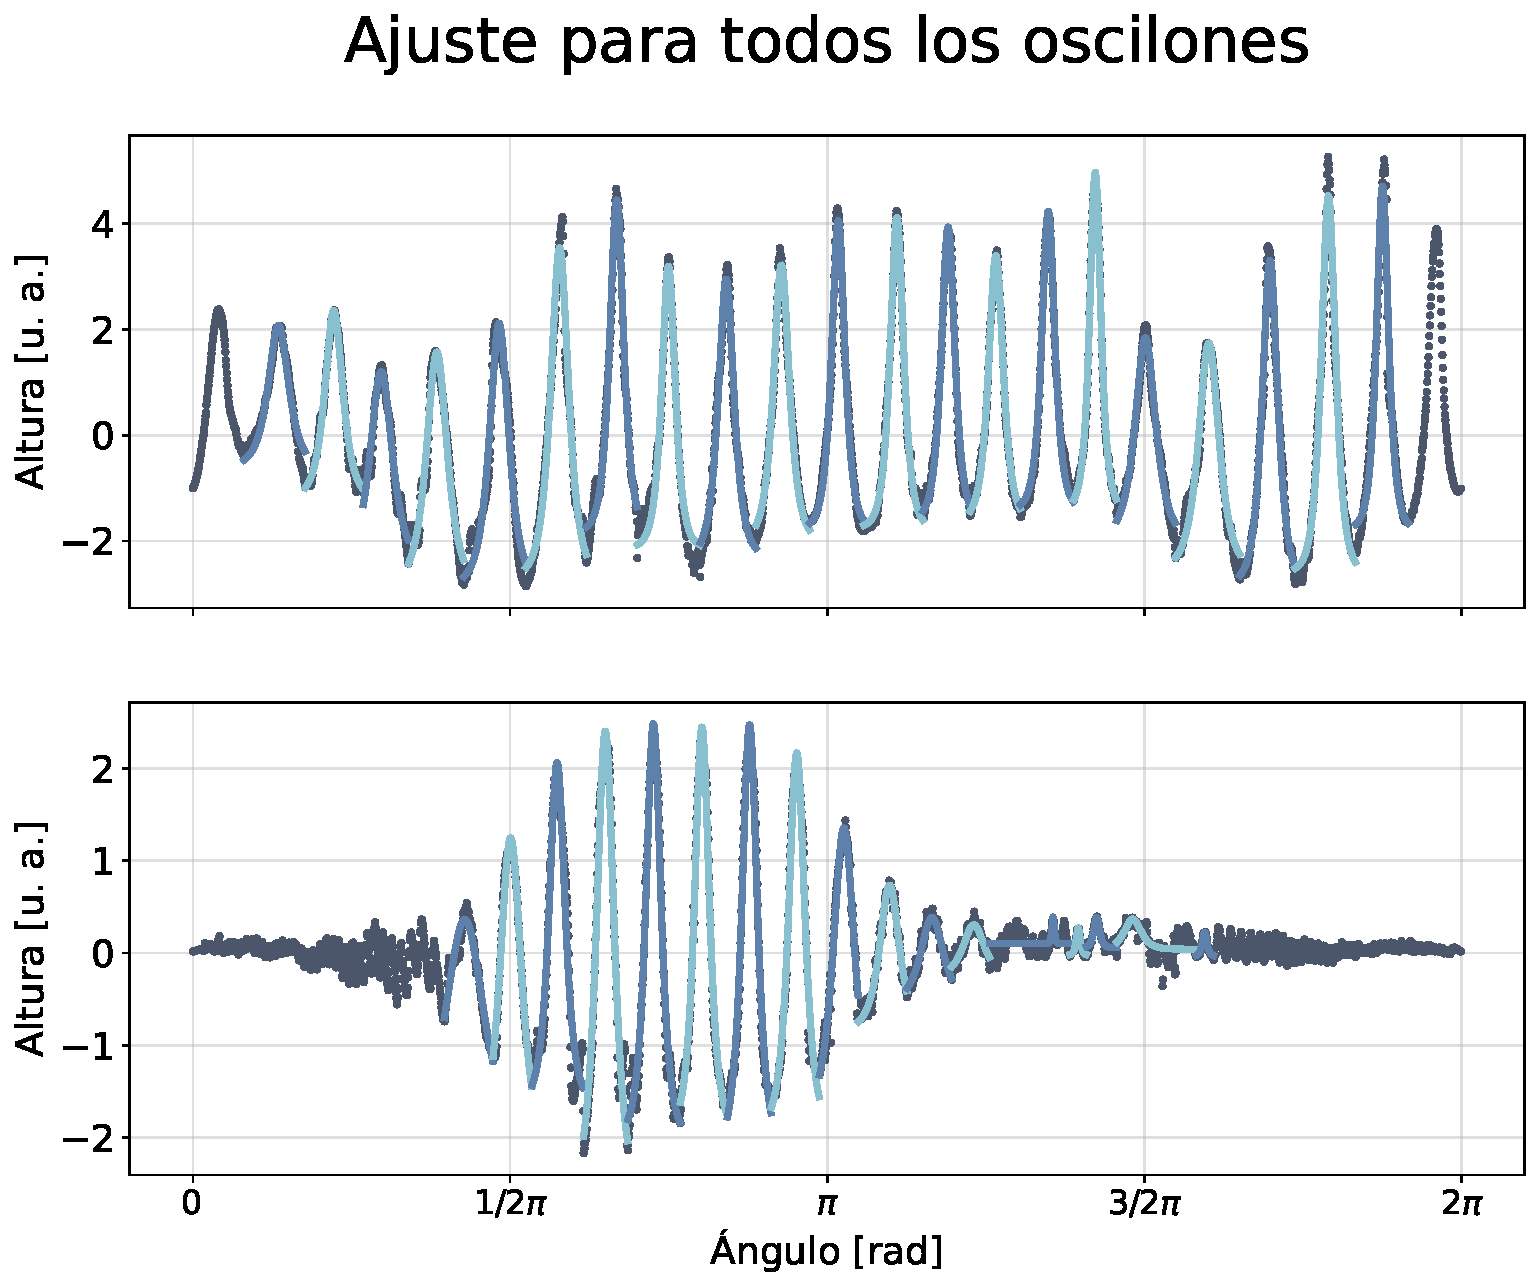
\includegraphics[width=\linewidth]{figs/fit_all_osc.pdf}
	  \end{figure}
	\end{minipage}
\end{frame}


\begin{frame}{Detección de la velocidad de los oscilones} % TODO
	\begin{figure}
		\centering
		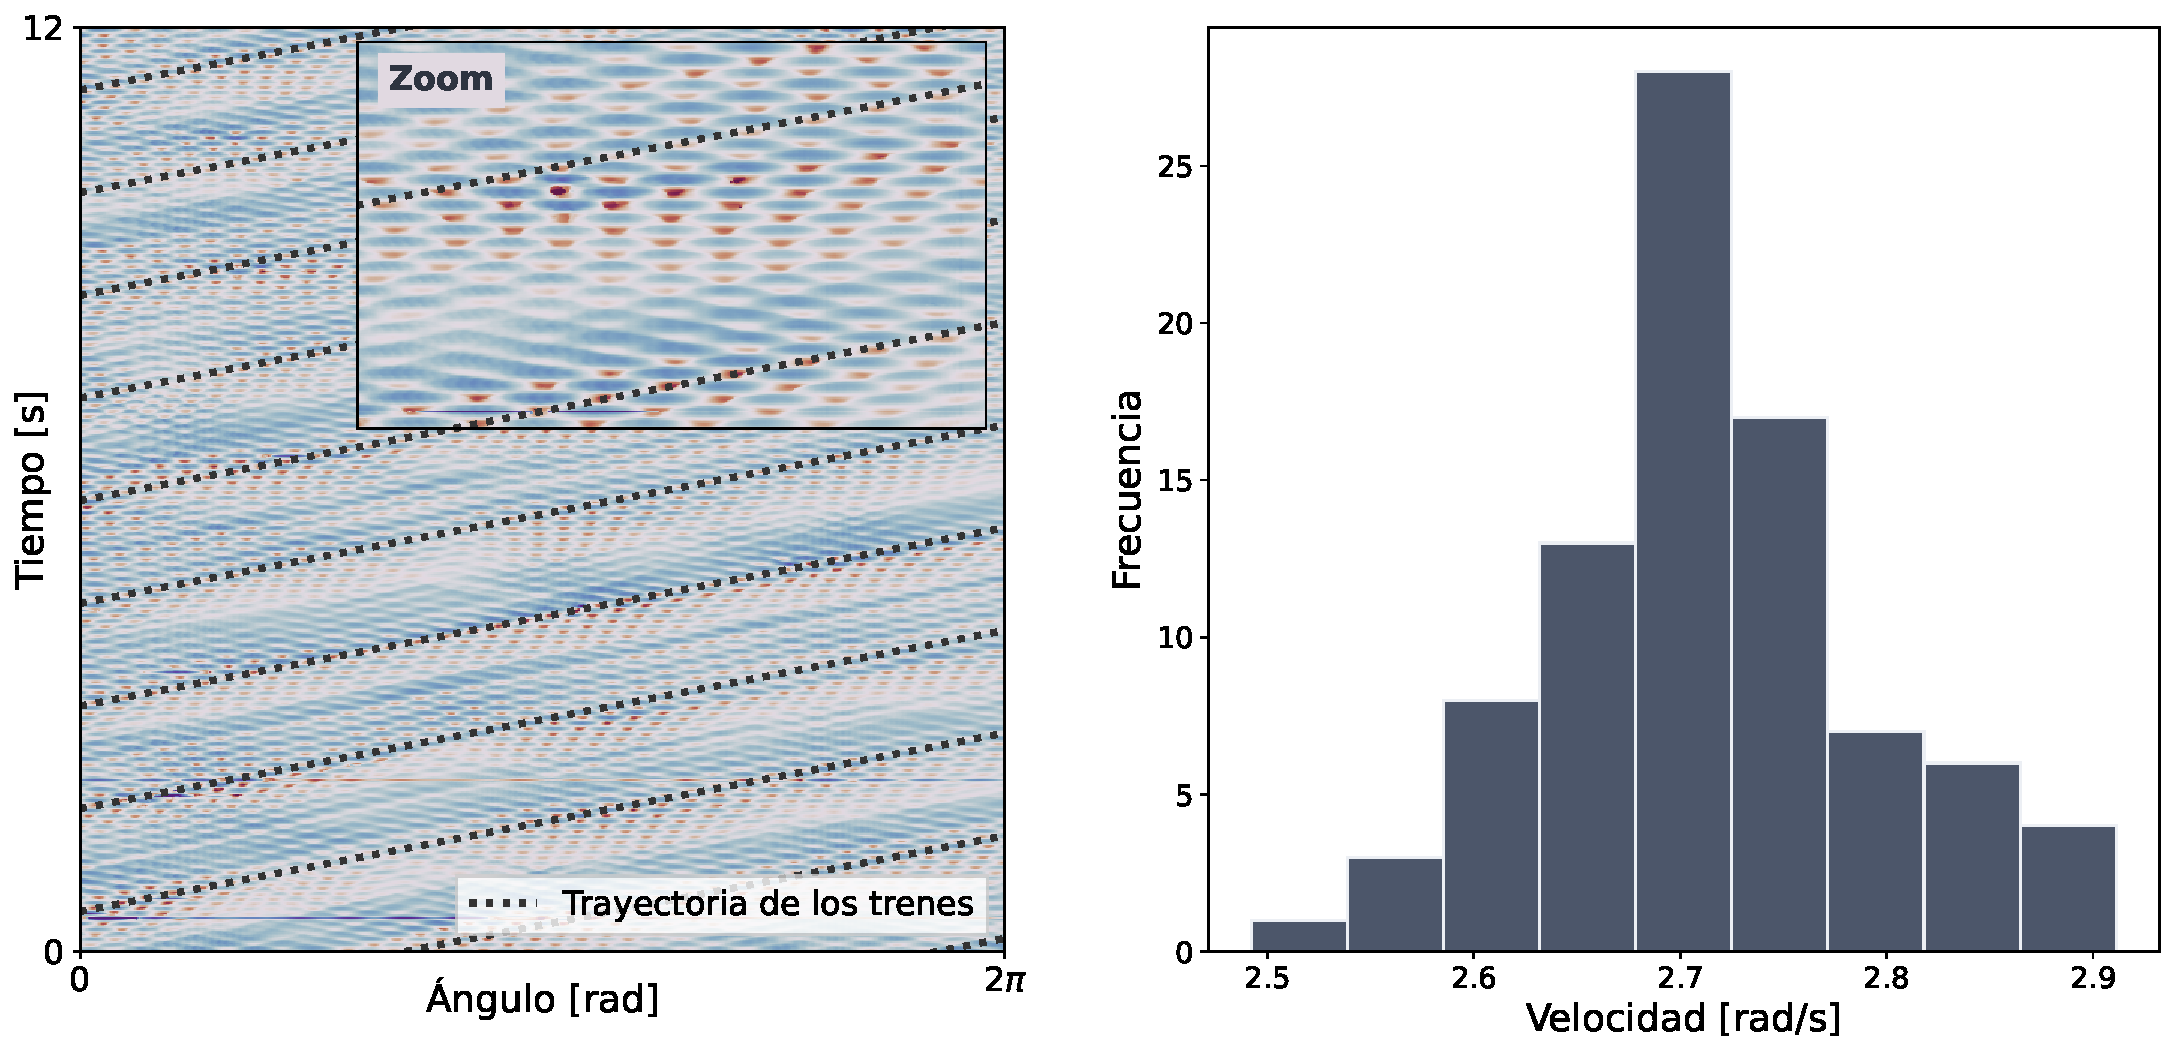
\includegraphics[width=\textwidth]{figs/velocidad_osc.pdf}
	\end{figure}
\end{frame}

\begin{frame}{Envolvente de la superficie libre} % TODO: Quizás otra diapo?
	\begin{figure}[ht]
		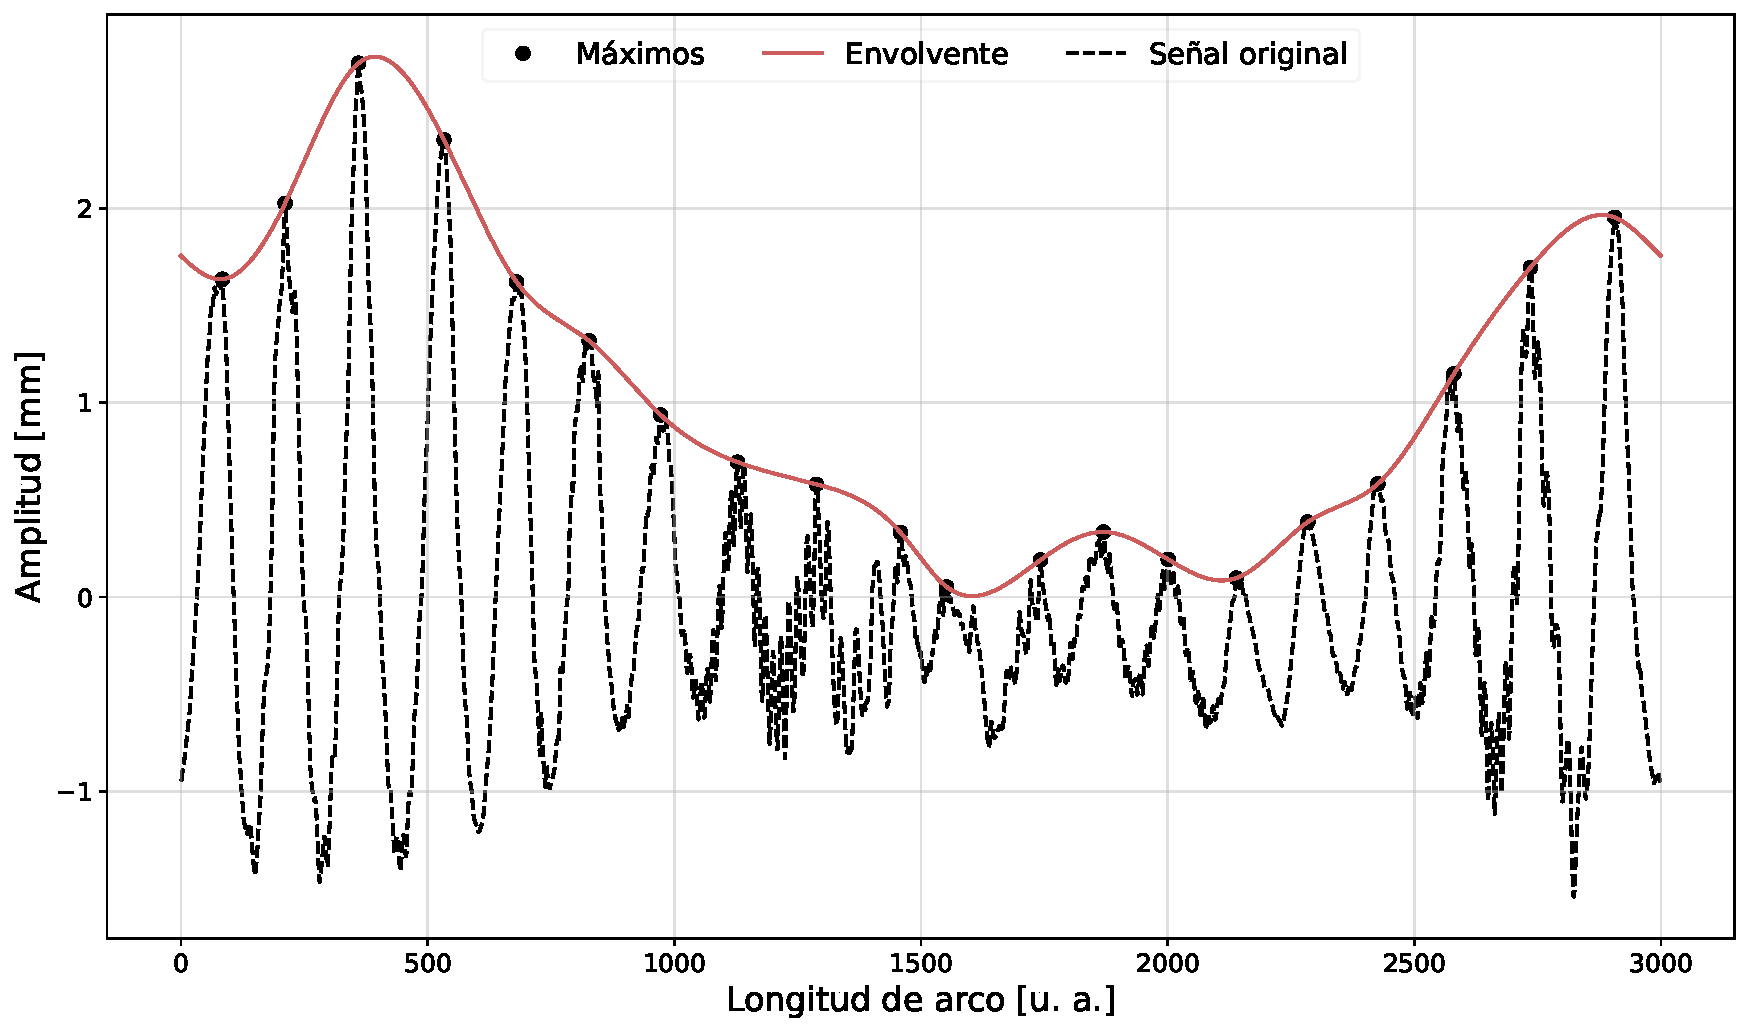
\includegraphics[width=0.9\textwidth]{figs/env_1sample.pdf}
	\end{figure}
	%TODO[berna]: Sacarle el fondo a la legend
\end{frame}

\begin{frame}{Envolvente de la superficie libre}
	\begin{figure}[ht]
		\centering
		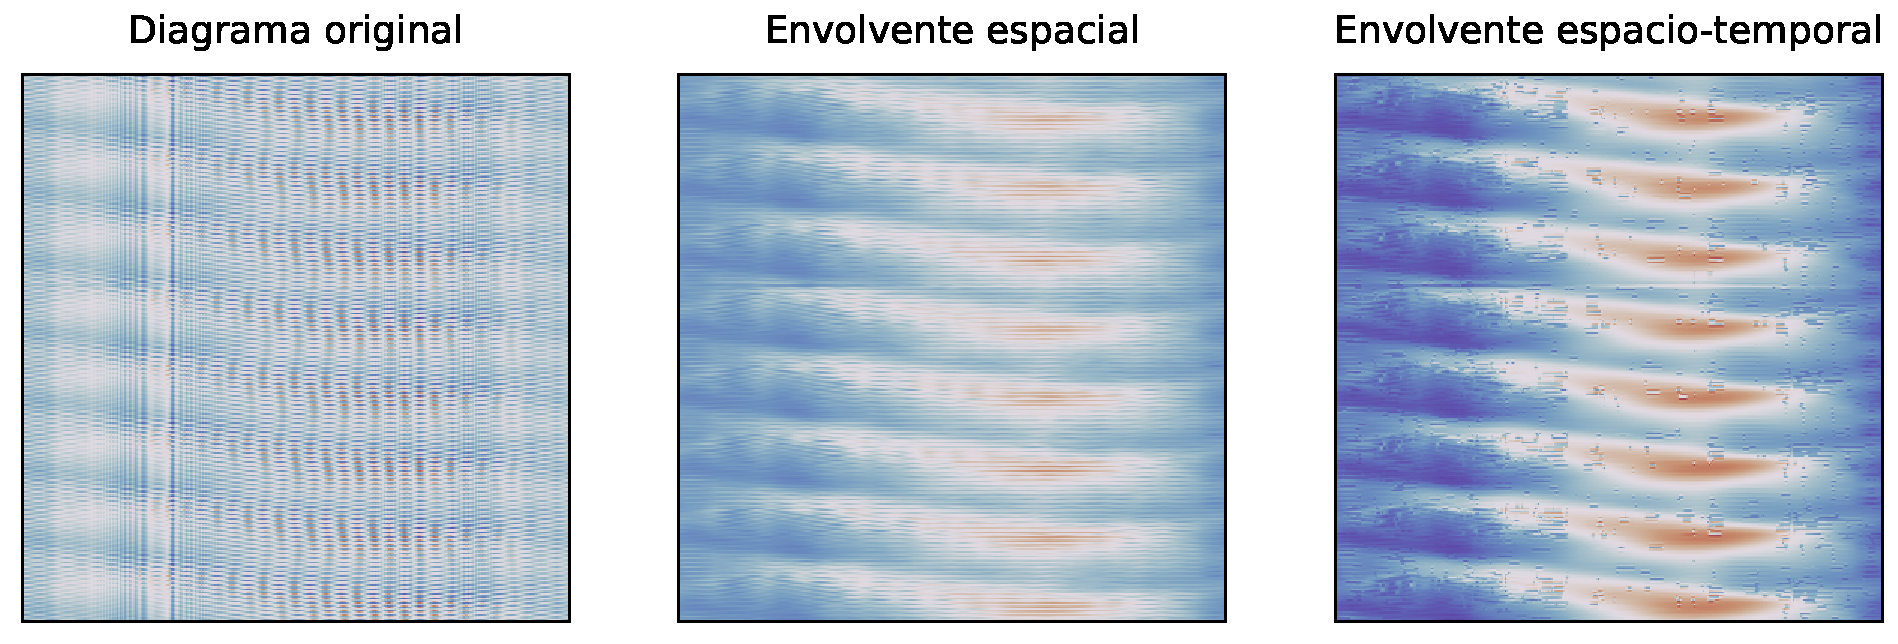
\includegraphics[width=\textwidth]{figs/st_envelopes.pdf}
	\end{figure}
\end{frame}

\begin{frame}{Inestabilidad de Taylor-Couette} % TODO
	\begin{minipage}{0.45\textwidth}
		\centering\small Esquema experimental
	  \begin{figure}
	    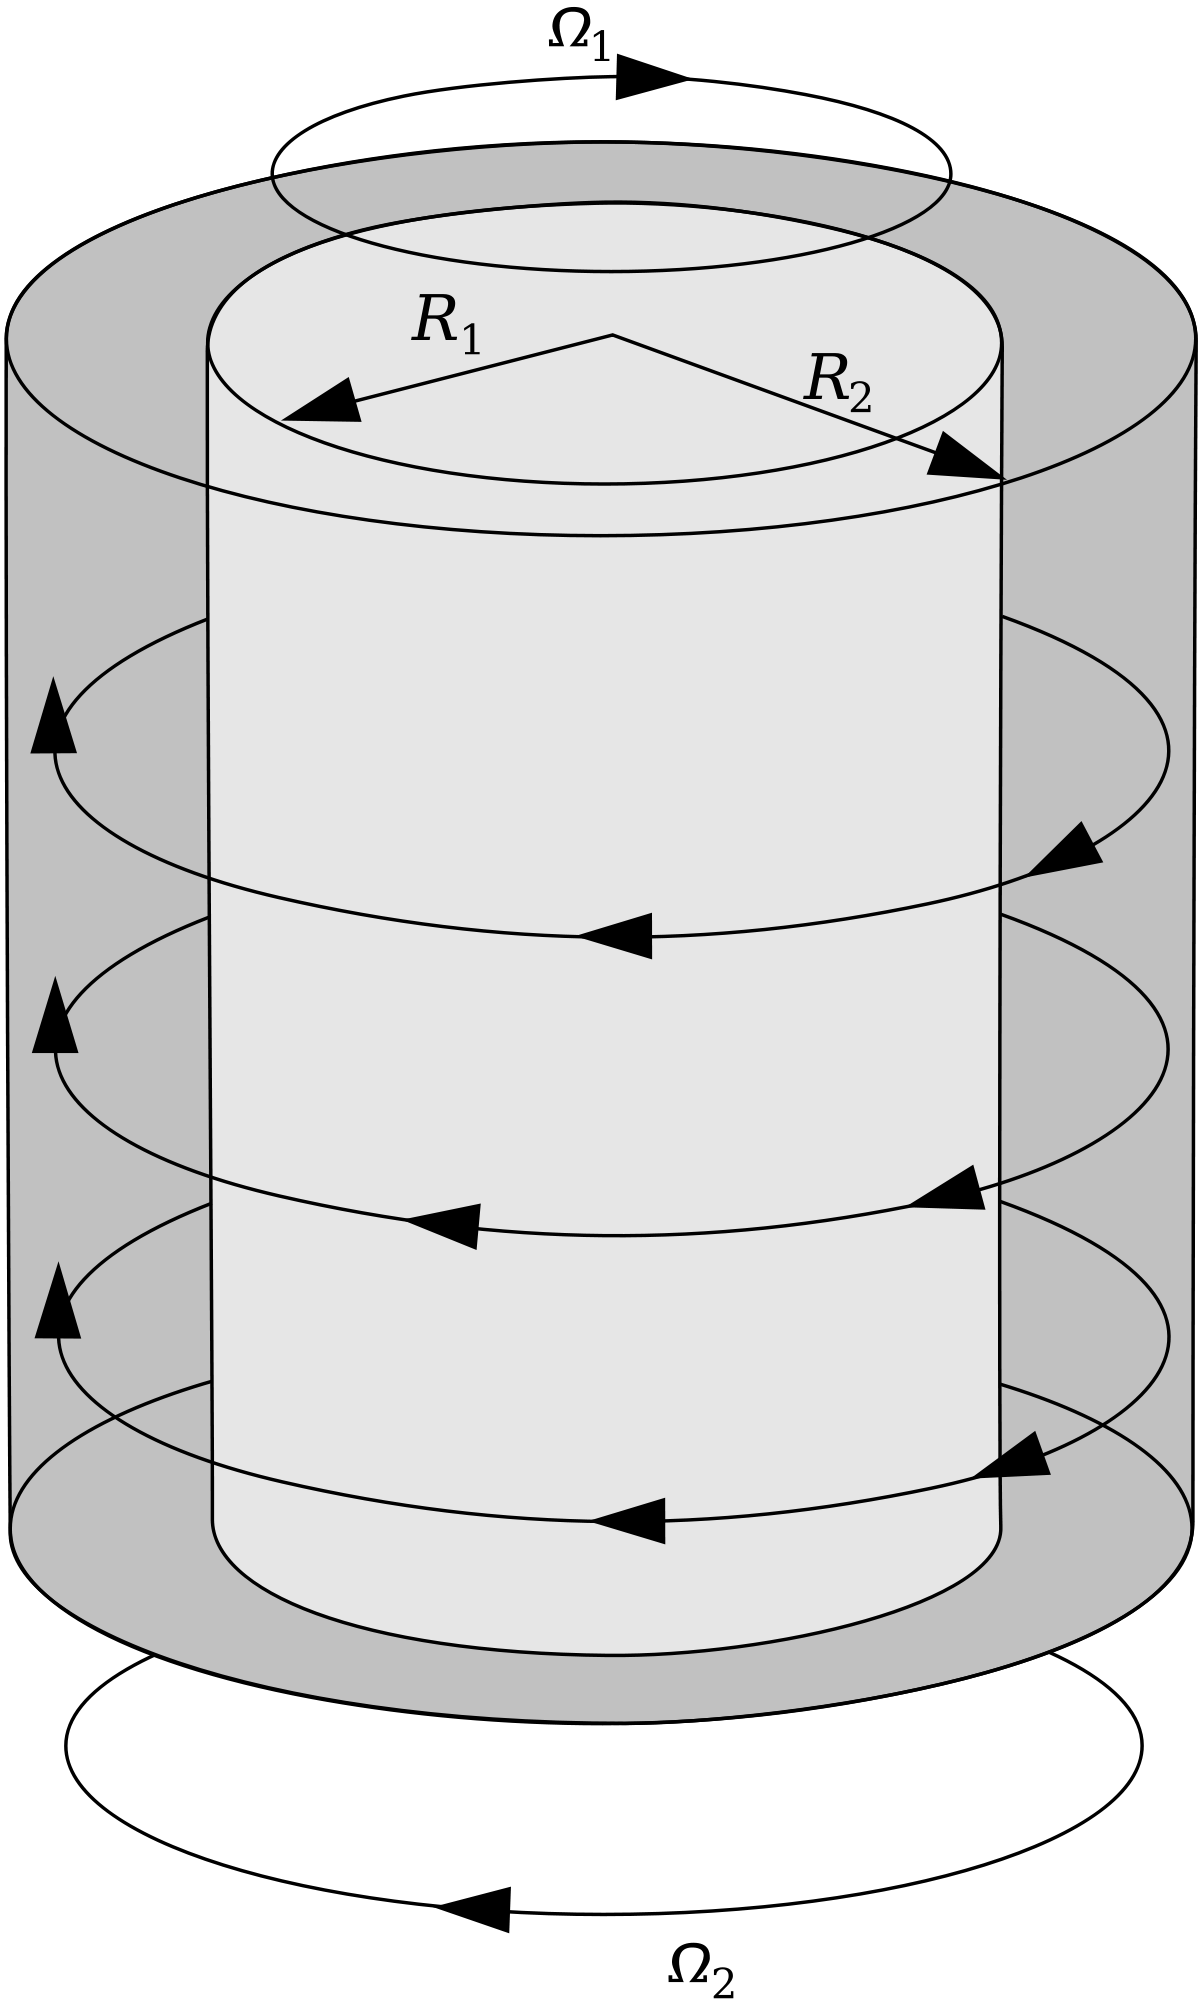
\includegraphics[width=0.535\linewidth]{figs/taylor_couette_diagram.png}
	  \end{figure}
	\end{minipage} \hfill
	\begin{minipage}{0.45\textwidth}
		\vskip-1.1em
		\centering\small Fotografía de la celda en rotación
	  \begin{figure}
	    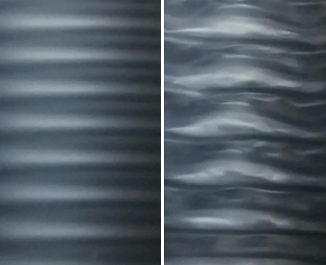
\includegraphics[width=\linewidth]{figs/taylor_couette.png}
	  \end{figure}
	\end{minipage}

	\hfill

	\tiny P. D. Weidman, “Measurement Techniques in Laboratory Rotating Flows” in Advances in Fluid Mechanics Measurements (Springer-Verlag, Heidelberg) 412–418 (1989).
\end{frame}


\begin{frame}{Inestabilidad de Taylor-Couette} % TODO
	\begin{minipage}{0.45\textwidth}
		\vskip-1.1em
		\centering\small Fotografía de la celda en rotación
	  \begin{figure}
	    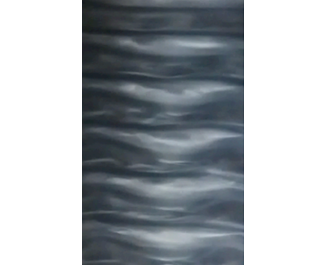
\includegraphics[width=\linewidth]{figs/taylor_couette_flipped.png}
	  \end{figure}
	\end{minipage} \hfill
	\begin{minipage}{0.45\textwidth}
		\centering\small ST para excitación vertical 
	  \begin{figure}
	    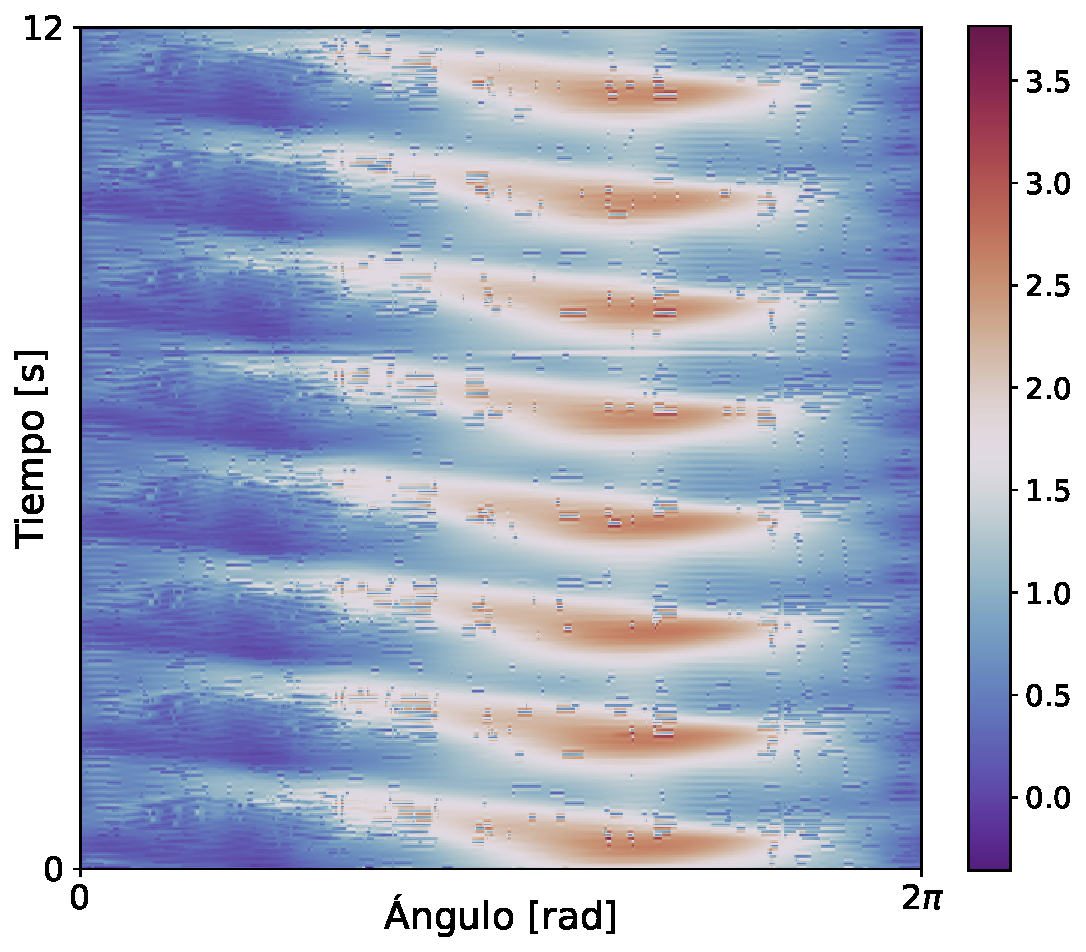
\includegraphics[width=\linewidth]{figs/st_taylor_couette.pdf}
	  \end{figure}
	\end{minipage}

	\hfill

	\tiny P. D. Weidman, “Measurement Techniques in Laboratory Rotating Flows” in Advances in Fluid Mechanics Measurements (Springer-Verlag, Heidelberg) 412–418 (1989).
\end{frame}

\begin{frame}{Ondas propagativas} % TODO: Ponerle alturas?
	\begin{figure}[ht]
		\centering
		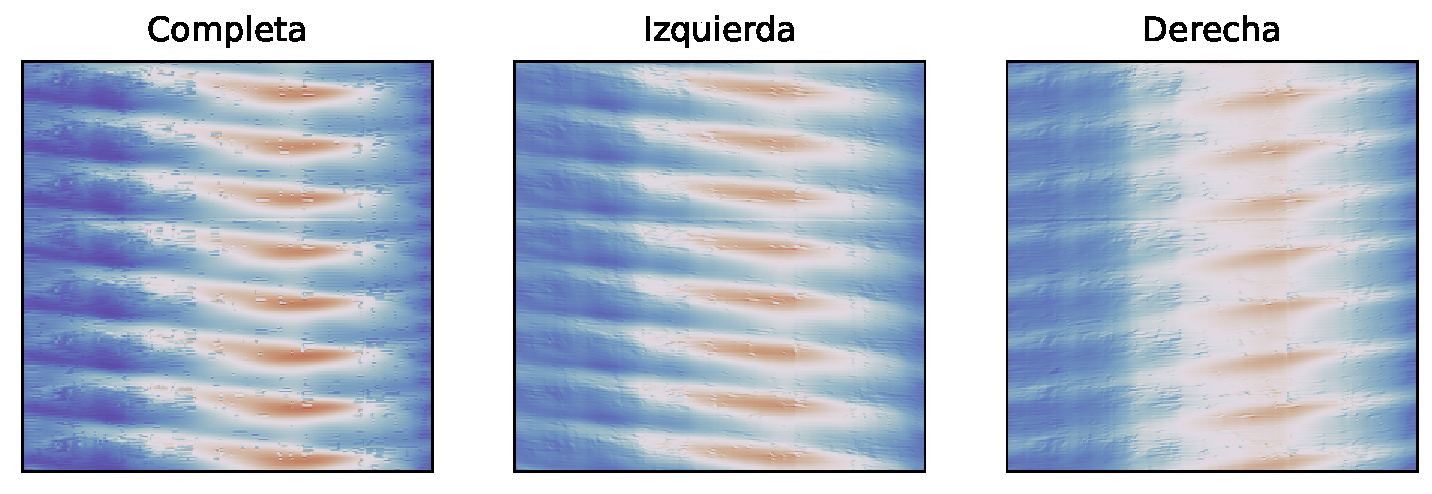
\includegraphics[width=\textwidth]{figs/st_left_right_taylor_couette.pdf}
	\end{figure}
\end{frame}

\begin{frame}{Ondas propagativas}
	\begin{figure}[ht]
		\centering
		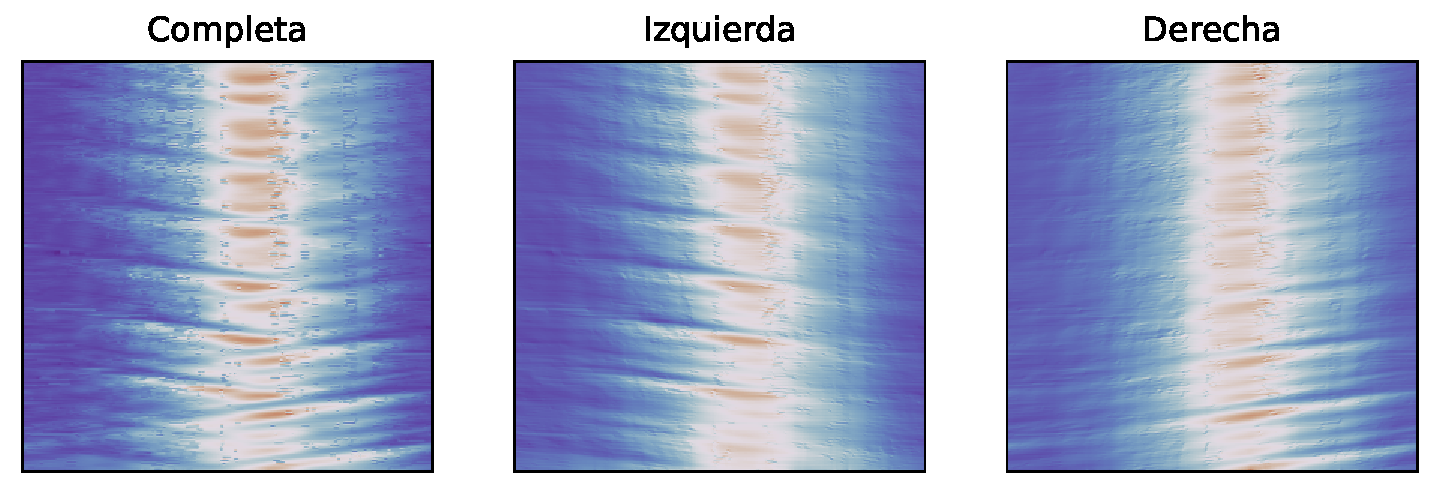
\includegraphics[width=\textwidth]{figs/st_left_right_med33.pdf}
	\end{figure}
\end{frame}

\begin{frame}{Relación de dispersión} % TODO: Las que vimos lineales y ver las de modulación de fase
	\begin{minipage}{0.46\textwidth}
	  \begin{figure}
		  \centering
	    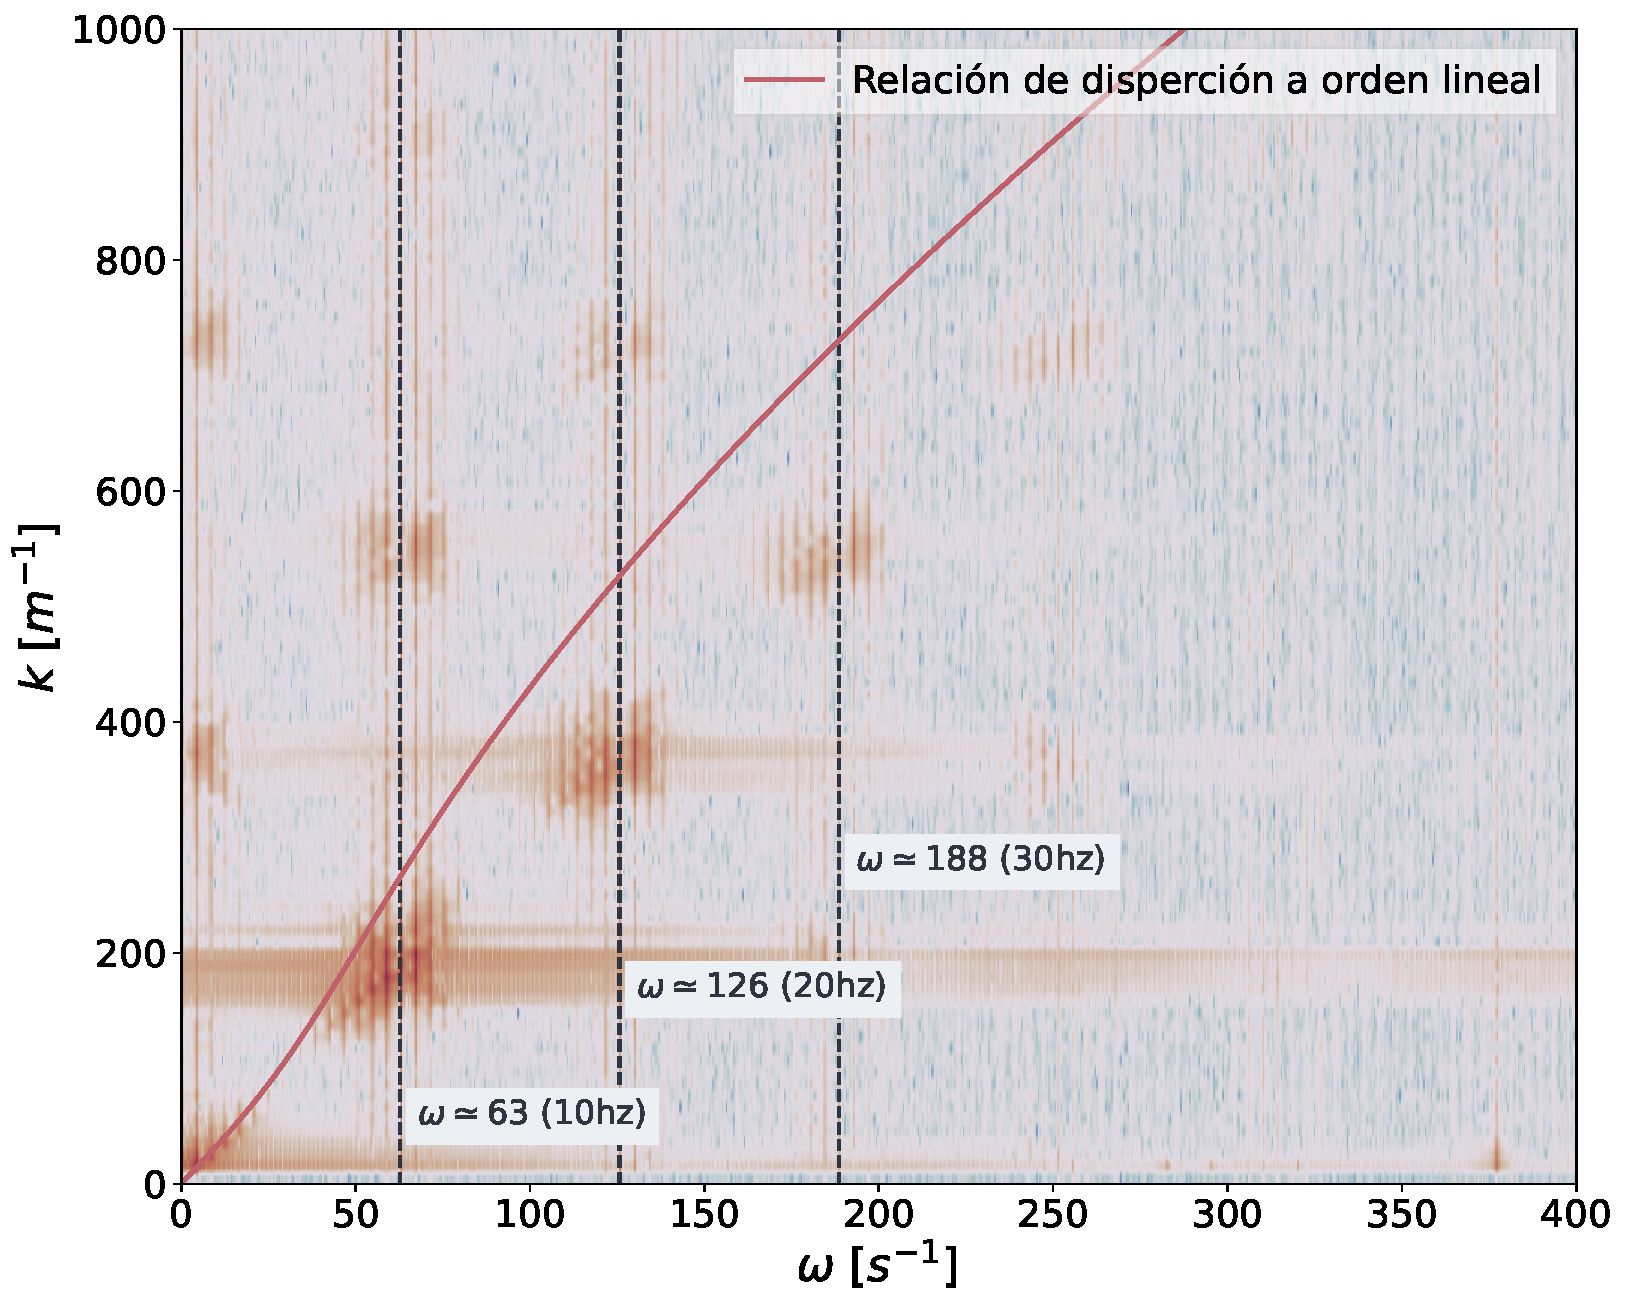
\includegraphics[width=\linewidth]{figs/dispersion_relation.pdf}
	  \end{figure}
	\end{minipage} \hfill
	\begin{minipage}{0.46\textwidth}
		\pause
	  \begin{figure}
	    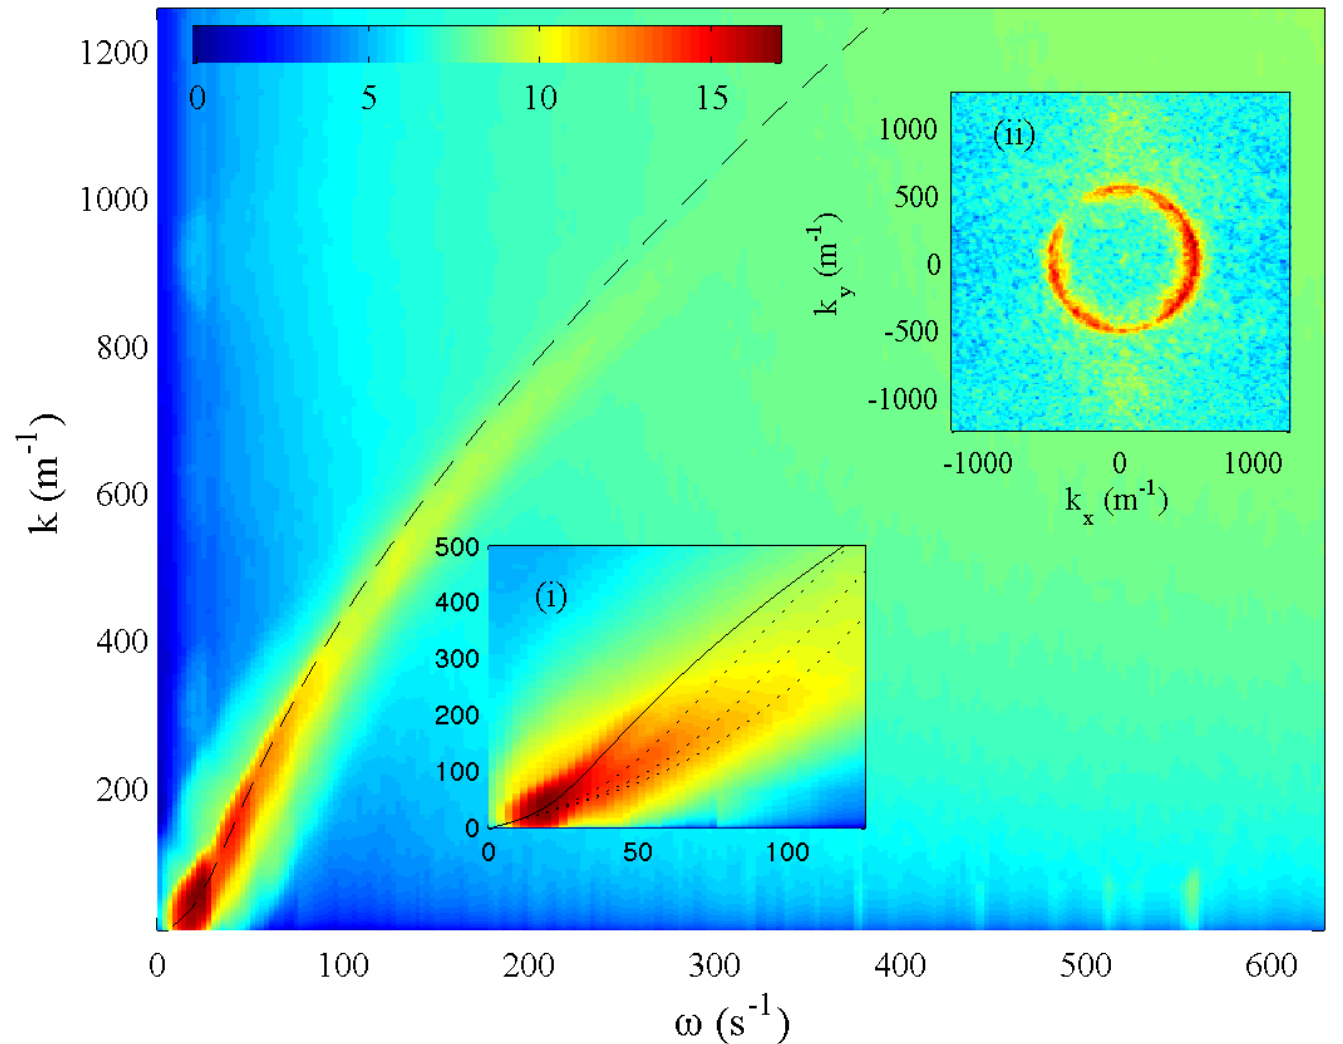
\includegraphics[width=\linewidth]{figs/dispersion_relation_cobelli.png}
	  \end{figure}
	\end{minipage}

	\vfill
	\tiny DER: P. J. Cobelli; A. Przadka; P. Petitjeans; G. Lagubeau; V. Pagneux; et al.; Different regimes for water wave turbulence; American Physical Society; Physical Review Letters; 107; 21; 11-2011; 1-5; 214503
\end{frame}


\section{Conclusiones}
\begin{frame}{Conclusiones}
	\textbf{Resultados}
	\begin{itemize} 
		\item Desarrollamos un método de medición robusto.
		\item Implementamos herramientas de análisis.
		\item Caracterizamos el sistema para distintos regímenes.
	\end{itemize}

	\hfill

	\textbf{Perspectivas}
	\begin{itemize} 
		\item Estudiar Taylor-Couette.
		\item Analizar dependencia de la velocidad con la amplitud.
		\item Ajustar la envolvente con ecuaciones de amplitud.
	\end{itemize}
\end{frame}

\section*{Gracias.}

\begin{frame}{Corrección de errores en los diagramas espacio-temporales}
	\begin{figure}
		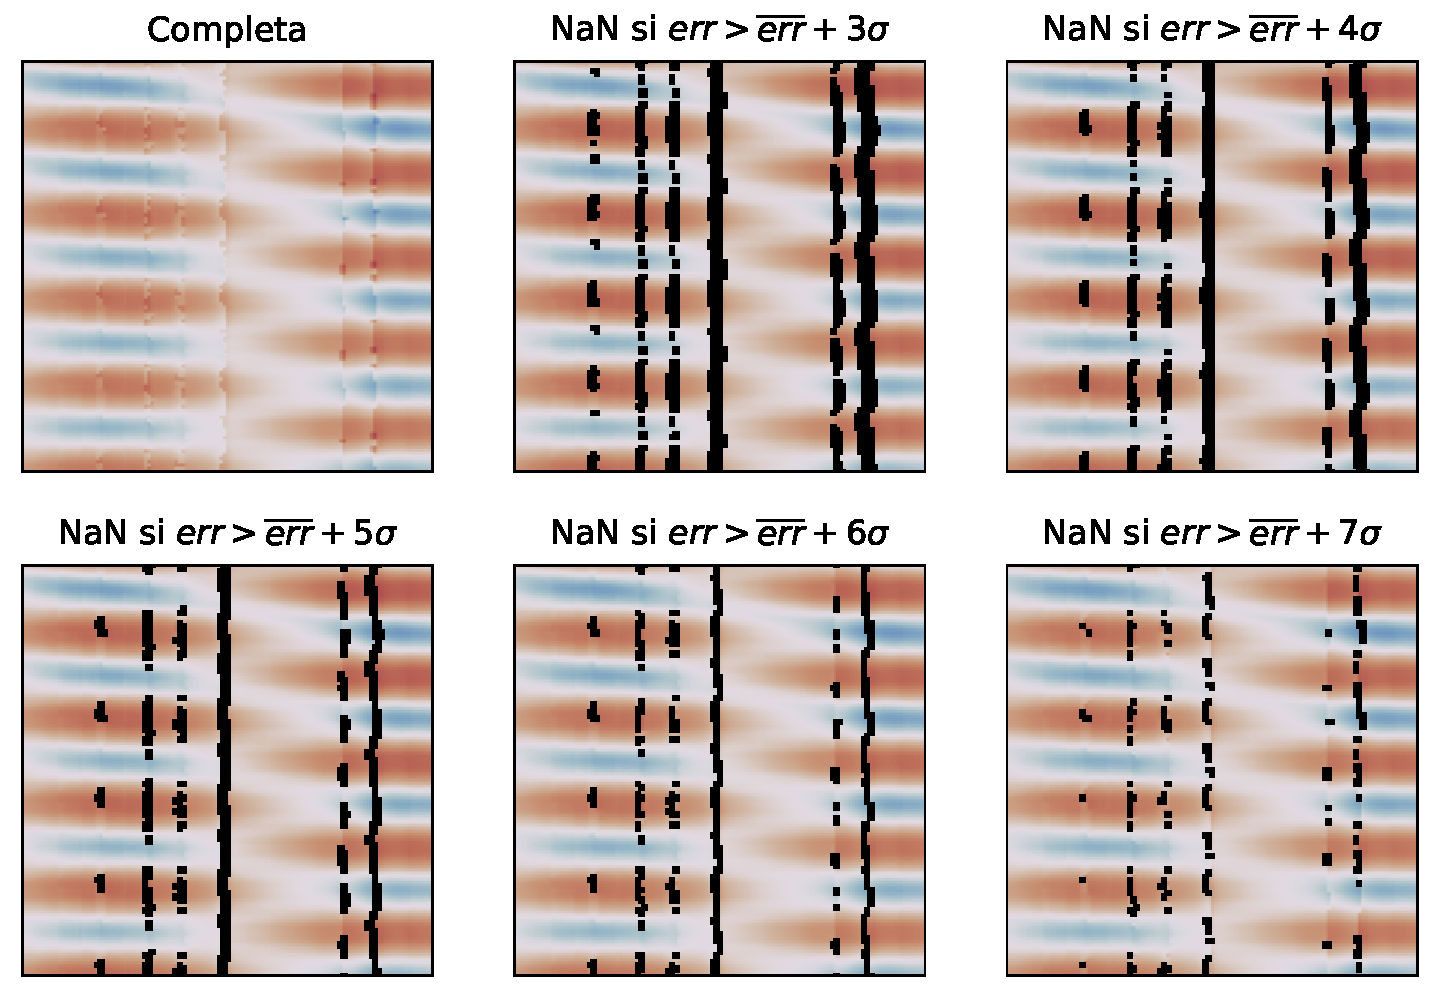
\includegraphics[width=0.75\linewidth]{figs/error_analysis.pdf}
	\end{figure}
\end{frame}

\begin{frame}{Corrección de errores en los diagramas espacio-temporales}
	\begin{figure}
		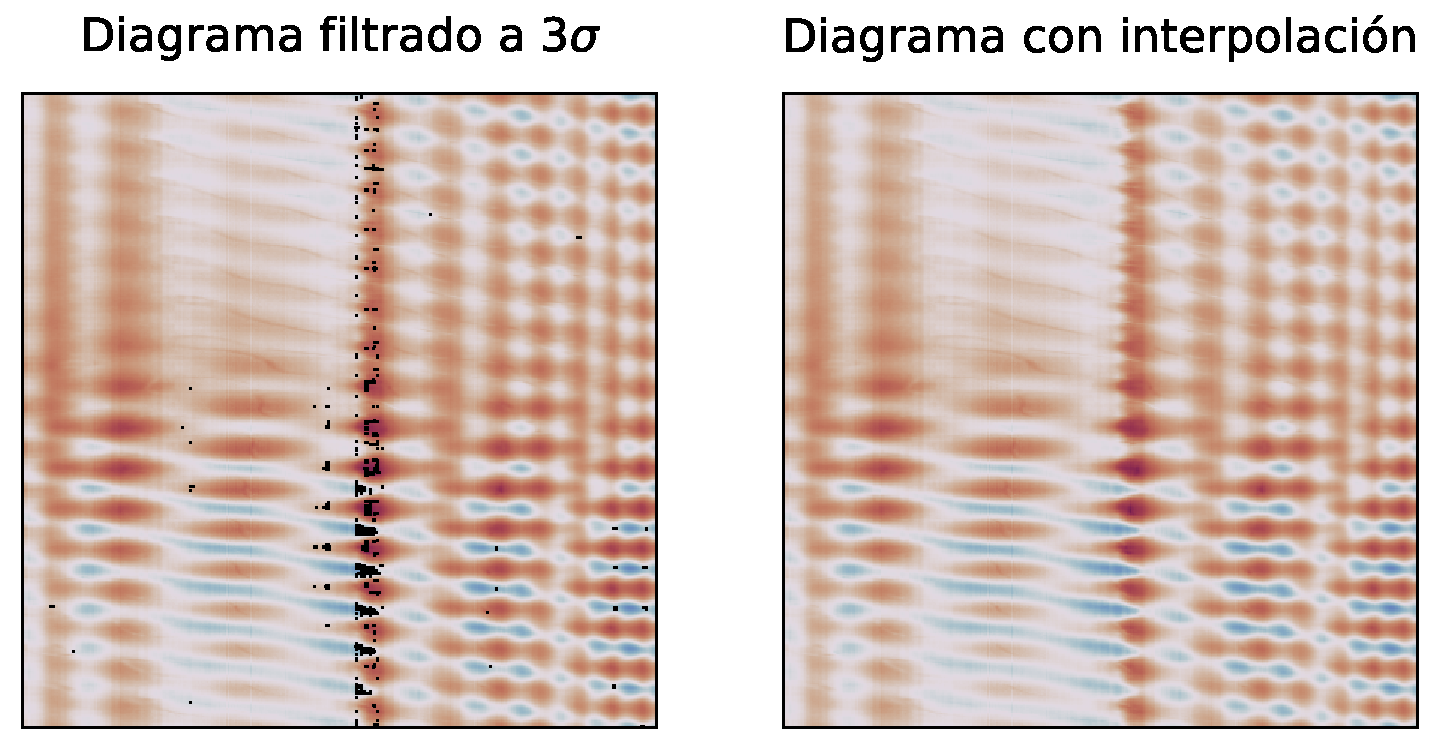
\includegraphics[width=0.8\linewidth]{figs/error_interp.pdf}
	\end{figure}
\end{frame}


\begin{frame}{Manejo de archivos y HDF5}
	\begin{figure}
		\centering
		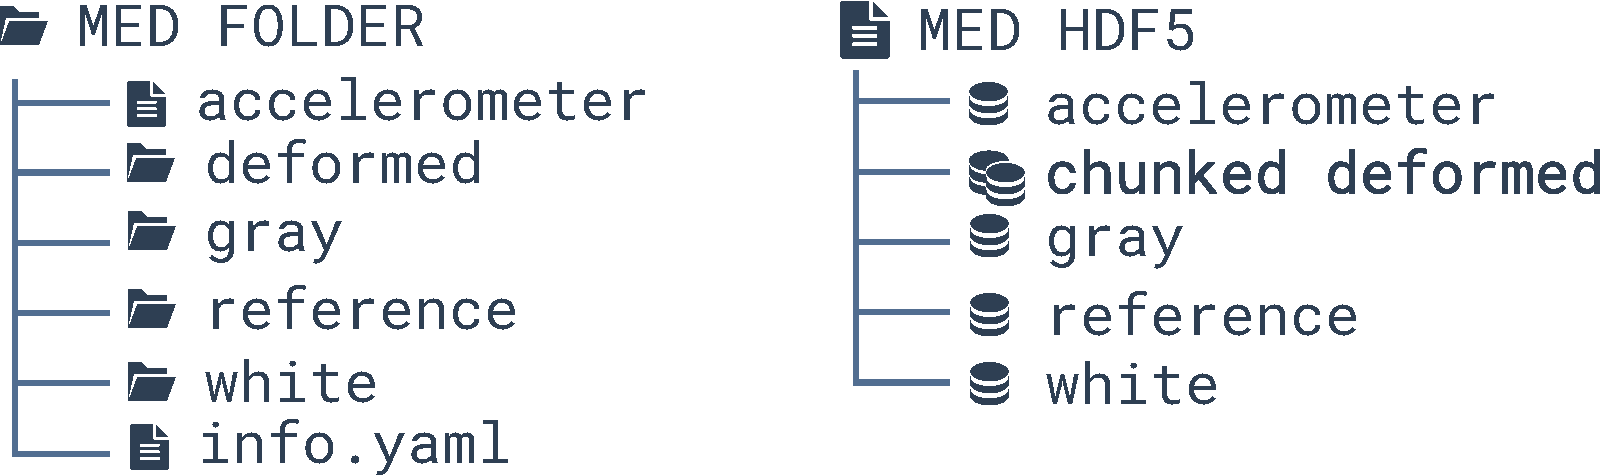
\includegraphics[width=1\textwidth]{figs/med_folder_to_hdf5.pdf}
	\end{figure}
\end{frame}

\begin{frame}{HDF5}
	\begin{figure}[ht]
		\centering
		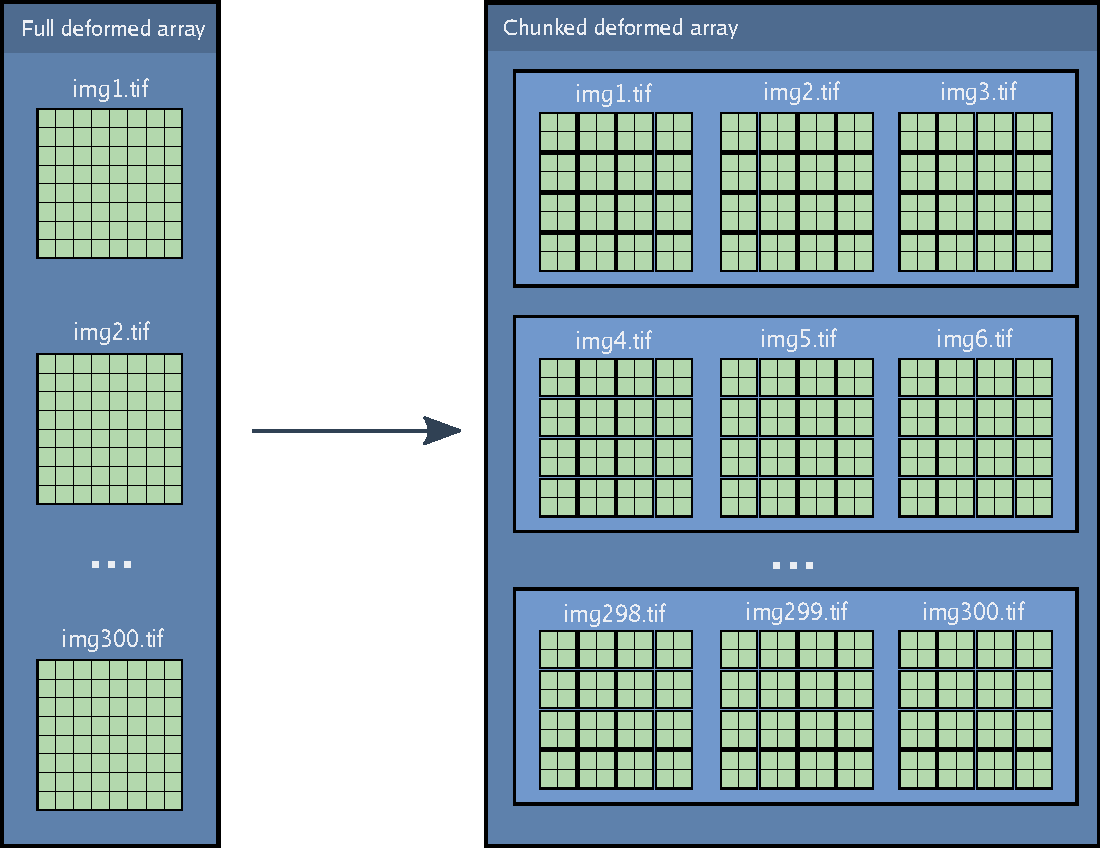
\includegraphics[width=0.7\textwidth]{figs/hdf5_chunk.pdf}
	\end{figure}
\end{frame}



\end{document}
